% ------------------------------------------------------------------
% Statistics booklet.
% GENERATED by src/build.py from src/content_statistics.py -- edit content_statistics.py and
% re-run the build, so every practice answer gets re-checked.
% ------------------------------------------------------------------
\documentclass[12pt,a4paper]{article}
\usepackage[a4paper,top=1.4cm,bottom=1.8cm,left=1.5cm,right=1.5cm,footskip=0.8cm]{geometry}
\usepackage[T1]{fontenc}
\usepackage[scaled=0.95]{helvet}
\renewcommand{\familydefault}{\sfdefault}
\usepackage{amsmath,amssymb}
\usepackage[table]{xcolor}
\usepackage[most]{tcolorbox}
\usepackage{enumitem,multicol,array,tabularx,pifont,fancyhdr,titlesec}

\definecolor{accent}{HTML}{1D6B8C}
\definecolor{accentlight}{HTML}{E3F0F6}
\definecolor{checkcol}{HTML}{8A3B12}
\definecolor{checklight}{HTML}{F6E7DE}
\definecolor{muted}{HTML}{56616B}
\definecolor{good}{HTML}{2E7D32}
\definecolor{warm}{HTML}{FFF6DD}
\definecolor{warmedge}{HTML}{E3B341}

\setlength{\parindent}{0pt}
\setlength{\parskip}{4pt}
\newcommand{\cmark}{\textcolor{good}{\ding{51}}}
\newcommand{\xmark}{\textcolor{red!70!black}{\ding{55}}}
\newcommand{\tickbox}{{\Large$\square$}}
\titleformat*{\subsection}{\large\bfseries\color{accent}}
\titlespacing*{\subsection}{0pt}{8pt}{4pt}

\pagestyle{fancy}
\fancyhf{}
\renewcommand{\headrulewidth}{0pt}
\fancyfoot[L]{\footnotesize\color{muted}Statistics}
\fancyfoot[R]{\footnotesize\color{muted}Page \thepage}

% --- boxes -----------------------------------------------------------------
\tcbset{base/.style={enhanced, arc=2mm, boxrule=0.8pt, left=3mm, right=3mm, top=1.5mm, bottom=1.5mm}}
\newtcolorbox{tipbox}[1]{base, fontupper=\large, colframe=accent, colback=white, before upper={\textbf{#1.}\ }}
\newtcolorbox{stepsbox}[1]{base, fontupper=\large, colframe=accent, colback=white, before upper={\textbf{#1}\par}}
\newtcolorbox{rememberbox}{base, fontupper=\large, colframe=warmedge, colback=warm, before upper={\textbf{Remember:}\ }}
\newenvironment{examples}{\begin{tcbraster}[raster columns=3, raster equal height=rows,
  raster column skip=2.5mm, raster row skip=2.5mm, raster before skip=2mm, raster after skip=3mm]}{\end{tcbraster}}
\newcommand{\example}[3]{\begin{tcolorbox}[base, colframe=black!25, colback=white, boxrule=0.5pt, arc=1.5mm]
  {\Large #1}\par\vspace{-2pt}{\color{black!25}\rule{\linewidth}{0.4pt}}\par
  {\normalsize\color{black!75}#2}\par\vspace{2pt}
  {\Large\color{good}\boldmath #3}\end{tcolorbox}}

\newcommand{\stepnum}[2]{\tikz[baseline=(n.base)]\node[circle,fill=#2,text=white,inner sep=0pt,
  minimum size=8mm,font=\large\bfseries](n){#1};}
\newcommand{\qnum}[1]{\tikz[baseline=(n.base)]\node[circle,fill=accentlight,text=accent,inner sep=0pt,
  minimum size=6mm,font=\small\bfseries](n){#1};}
\newcommand{\cnum}[1]{\tikz[baseline=(n.base)]\node[circle,fill=checklight,text=checkcol,inner sep=0pt,
  minimum size=6.5mm,font=\small\bfseries](n){#1};}

% \banner{number}{title}{label}{colour}
\newcommand{\banner}[4]{\begin{tcolorbox}[enhanced, colback=#4, colframe=#4, arc=2mm,
  left=3mm, right=3mm, top=2mm, bottom=2mm, after skip=3mm]
  \color{white}\tikz[baseline=(n.base)]\node[circle,fill=white,text=#4,inner sep=0pt,
  minimum size=8.5mm,font=\Large\bfseries](n){#1};\hspace{3mm}{\LARGE\bfseries #2}\hfill
  \colorbox{white!20!#4}{\bfseries\MakeUppercase{#3}}\end{tcolorbox}}

% \qbox{n}{question}{height}
\newcommand{\qbox}[3]{\begin{tcolorbox}[base, height=#3, text fill, colframe=black!30, colback=white, boxrule=0.5pt,
  arc=1.5mm, top=1.5mm, bottom=2mm]\qnum{#1}\hspace{2.5mm}{\Large #2}\par\vfill
  {\Large$=$}\hspace{2mm}\textcolor{black!45}{\rule{0.8\linewidth}{0.6pt}}\end{tcolorbox}}

% \cbox{n}{question}{height}  -- skill check question, with a mark box
\newcommand{\cbox}[3]{\begin{tcolorbox}[base, height=#3, text fill, colframe=checkcol!70, colback=white, boxrule=0.8pt,
  arc=1.5mm, left=2mm, right=2mm, top=1.5mm, bottom=2mm]\cnum{#1}\hfill
  \fcolorbox{checkcol}{white}{\rule{0pt}{4.5mm}\hspace{4.5mm}}\par\vspace{1mm}
  {\large #2}\par\vfill
  {\large$=$}\hspace{1mm}\textcolor{black!45}{\rule{0.8\linewidth}{0.6pt}}\end{tcolorbox}}

% \checkhead{n}{title}{instruction}{marks}
\newcommand{\checkhead}[4]{\begin{tcolorbox}[enhanced, colback=checklight, colframe=checklight, arc=1.5mm,
  left=2mm, right=2mm, top=0.8mm, bottom=0.8mm, before skip=4mm, after skip=2mm]
  \cnum{#1}\hspace{2mm}\textbf{\color{checkcol}#2}\quad #3\hfill
  \textbf{\color{checkcol}Mark: \underline{\hspace{8mm}} / #4}\end{tcolorbox}}

\newcommand{\fillline}[1]{\textcolor{black}{\rule{#1}{0.6pt}}}
\newcommand{\ansline}[1]{\textcolor{black!45}{\rule{#1\linewidth}{0.6pt}}}

% \pbox[options]{n}{height}{body} -- a practice question of any type
\newcommand{\pbox}[4][]{\begin{tcolorbox}[base, height=#3, text fill, colframe=black!30, colback=white, boxrule=0.5pt,
  arc=1.5mm, top=1.5mm, bottom=2mm, #1]\qnum{#2}\hspace{2.5mm}#4\end{tcolorbox}}
% \kbox[options]{n}{height}{body} -- a skill check question of any type, with a mark box
\newcommand{\kbox}[4][]{\begin{tcolorbox}[base, height=#3, text fill, colframe=checkcol!70, colback=white, boxrule=0.8pt,
  arc=1.5mm, left=2mm, right=2mm, top=1.5mm, bottom=2mm, #1]\cnum{#2}\hfill
  \fcolorbox{checkcol}{white}{\rule{0pt}{4.5mm}\hspace{4.5mm}}\par\vspace{1mm}#4\end{tcolorbox}}

\begin{document}

\thispagestyle{empty}
\begin{tcolorbox}[enhanced, colback=accent, colframe=accent, arc=3mm, halign=center, top=12mm, bottom=11mm]
\color{white}{\small\bfseries S\,T\,A\,T\,I\,S\,T\,I\,C\,S\quad W\,O\,R\,K\,B\,O\,O\,K}\par\vspace{3mm}
{\fontsize{34}{40}\selectfont\bfseries Statistics}\par\vspace{3mm}
{\Large Collect it. Show it. Make sense of it.}
\end{tcolorbox}
\vspace{10mm}
{\large Name: \fillline{9.5cm} \hfill Class: \fillline{3.5cm}}

\vspace{12mm}
{\Large\bfseries\color{accent} My progress}\par\vspace{2mm}
\renewcommand{\arraystretch}{2.1}
\begin{tabularx}{\linewidth}{|c|X|c|p{2.4cm}|}
\hline
\rowcolor{accentlight} & \textbf{Skill} & \small\textbf{Practice done} & \small\textbf{Skill Check} \\ \hline
\textbf{\color{accent}\large 1} & \textbf{Data Sources and Types}\newline {\small\color{muted}I can tell primary from secondary data, and categorical from numerical data} & \tickbox & \hfill/\,4 \\ \hline
\textbf{\color{accent}\large 2} & \textbf{Data Displays}\newline {\small\color{muted}I can name a data display and choose the best one for some data} & \tickbox & \hfill/\,4 \\ \hline
\textbf{\color{accent}\large 3} & \textbf{Scatter Plots}\newline {\small\color{muted}I can describe a point in context, and the strength of a scatter plot} & \tickbox & \hfill/\,3 \\ \hline
\textbf{\color{accent}\large 4} & \textbf{Lines of Best Fit}\newline {\small\color{muted}I can draw a line of best fit and use it to make a prediction} & \tickbox & \hfill/\,3 \\ \hline
\textbf{\color{accent}\large 5} & \textbf{Mean, Median and Mode}\newline {\small\color{muted}I can find the mean, median and mode of a set of data} & \tickbox & \hfill/\,4 \\ \hline
\textbf{\color{accent}\large 6} & \textbf{Range and Quartiles}\newline {\small\color{muted}I can find the range, LQ, UQ and IQR of a set of data} & \tickbox & \hfill/\,4 \\ \hline
\multicolumn{3}{r|}{\textbf{Skill Check total}} & \hfill/\,22 \\ \cline{4-4}
\end{tabularx}
\newpage
\banner{1}{Data Sources and Types}{Learn}{accent}
\begin{tcolorbox}[enhanced, colback=accentlight, colframe=accent, boxrule=0pt, leftrule=1.5mm, arc=0mm, top=1.5mm, bottom=1.5mm]\textbf{Goal:} I can tell primary from secondary data, and categorical from numerical data\end{tcolorbox}
\large

\subsection*{Where does the data come from?}
\begin{center}
\renewcommand{\arraystretch}{1.25}
\begin{tabular}{|p{3.4cm}|p{6.1cm}|p{6.2cm}|}
\hline
\rowcolor{accentlight} & \textbf{What it means} & \textbf{Examples} \\ \hline
\textbf{Primary data} & You collect it \textbf{yourself}. & A survey you give your class; measuring heights; counting cars. \\ \hline
\textbf{Secondary data} & \textbf{Someone else} collected it. & A website, a newspaper, Stats NZ, a book, last year's survey. \\ \hline
\end{tabular}
\end{center}

\subsection*{What type of data is it?}
\begin{center}
\renewcommand{\arraystretch}{1.25}
\begin{tabular}{|p{3.4cm}|p{6.1cm}|p{6.2cm}|}
\hline
\rowcolor{accentlight}\textbf{Type} & \textbf{What it means} & \textbf{Examples} \\ \hline
\textbf{Categorical} & Words or groups, not numbers. & Favourite food, eye colour, type of pet. \\ \hline
\textbf{Discrete numerical} & Numbers you \textbf{count}. Usually whole numbers. & Number of pets, goals scored, people in a family. \\ \hline
\textbf{Continuous numerical} & Numbers you \textbf{measure}. Can have decimals. & Height, weight, time, temperature. \\ \hline
\end{tabular}
\end{center}

\begin{tipbox}{Ask yourself two questions}
1. Is the answer a \textbf{word} or a \textbf{number}? A word means \textbf{categorical}.\\
2. If it is a number, did you \textbf{count} it (\textbf{discrete}) or \textbf{measure} it (\textbf{continuous})?
\end{tipbox}

\subsection*{Worked examples}
\begin{examples}
\example{\text{Favourite sport}}{The answers are words like \textquotedblleft{}rugby\textquotedblright{}}{\textbf{Categorical}}
\example{\text{Number of siblings}}{You count them: 0, 1, 2, 3\ldots}{\textbf{Discrete}}
\example{\text{Time to run 100\,m}}{You measure it: 14.6 seconds}{\textbf{Continuous}}
\end{examples}

\newpage\normalsize
\banner{1}{Data Sources and Types}{Practice}{accent}
{\large\textbf{Circle the correct answer.}} {\color{muted}Show your working in each box.}\par\vspace{1mm}
\begin{tcbraster}[raster columns=2, raster column skip=4mm, raster row skip=3mm]
\pbox{1}{3.1cm}{{\large Mere counts the cars that drive past the school gate in 10 minutes.}\par\vfill {\small Circle one:}\par\vspace{1mm}{\small\raggedright \fbox{\strut\ Primary\ }\quad \fbox{\strut\ Secondary\ }}}
\pbox{2}{3.1cm}{{\large Josh finds the populations of NZ cities on the Stats NZ website.}\par\vfill {\small Circle one:}\par\vspace{1mm}{\small\raggedright \fbox{\strut\ Primary\ }\quad \fbox{\strut\ Secondary\ }}}
\pbox{3}{3.1cm}{{\large Ana measures the heights of everyone in her class.}\par\vfill {\small Circle one:}\par\vspace{1mm}{\small\raggedright \fbox{\strut\ Primary\ }\quad \fbox{\strut\ Secondary\ }}}
\pbox{4}{3.1cm}{{\large Tom uses rainfall data from a weather website.}\par\vfill {\small Circle one:}\par\vspace{1mm}{\small\raggedright \fbox{\strut\ Primary\ }\quad \fbox{\strut\ Secondary\ }}}
\pbox{5}{3.1cm}{{\large Our class uses survey results that another class collected last year.}\par\vfill {\small Circle one:}\par\vspace{1mm}{\small\raggedright \fbox{\strut\ Primary\ }\quad \fbox{\strut\ Secondary\ }}}
\pbox{6}{3.1cm}{{\large Type of data: \textbf{favourite sport}}\par\vfill {\small Circle one:}\par\vspace{1mm}{\small\raggedright \fbox{\strut\ Categorical\ }\quad \fbox{\strut\ Discrete numerical\ }\quad \fbox{\strut\ Continuous numerical\ }}}
\pbox{7}{3.1cm}{{\large Type of data: \textbf{number of pets}}\par\vfill {\small Circle one:}\par\vspace{1mm}{\small\raggedright \fbox{\strut\ Categorical\ }\quad \fbox{\strut\ Discrete numerical\ }\quad \fbox{\strut\ Continuous numerical\ }}}
\pbox{8}{3.1cm}{{\large Type of data: \textbf{time to run 100\,m}}\par\vfill {\small Circle one:}\par\vspace{1mm}{\small\raggedright \fbox{\strut\ Categorical\ }\quad \fbox{\strut\ Discrete numerical\ }\quad \fbox{\strut\ Continuous numerical\ }}}
\pbox{9}{3.1cm}{{\large Type of data: \textbf{eye colour}}\par\vfill {\small Circle one:}\par\vspace{1mm}{\small\raggedright \fbox{\strut\ Categorical\ }\quad \fbox{\strut\ Discrete numerical\ }\quad \fbox{\strut\ Continuous numerical\ }}}
\pbox{10}{3.1cm}{{\large Type of data: \textbf{goals scored in a game}}\par\vfill {\small Circle one:}\par\vspace{1mm}{\small\raggedright \fbox{\strut\ Categorical\ }\quad \fbox{\strut\ Discrete numerical\ }\quad \fbox{\strut\ Continuous numerical\ }}}
\pbox{11}{3.1cm}{{\large Type of data: \textbf{weight of a newborn baby}}\par\vfill {\small Circle one:}\par\vspace{1mm}{\small\raggedright \fbox{\strut\ Categorical\ }\quad \fbox{\strut\ Discrete numerical\ }\quad \fbox{\strut\ Continuous numerical\ }}}
\pbox{12}{3.1cm}{{\large Type of data: \textbf{texts sent in a day}}\par\vfill {\small Circle one:}\par\vspace{1mm}{\small\raggedright \fbox{\strut\ Categorical\ }\quad \fbox{\strut\ Discrete numerical\ }\quad \fbox{\strut\ Continuous numerical\ }}}
\end{tcbraster}
\vfill\centerline{\color{good}\bfseries \ding{51}\ Check your answers at the back. Fix any you got wrong.}
\newpage
\banner{2}{Data Displays}{Learn}{accent}
\begin{tcolorbox}[enhanced, colback=accentlight, colframe=accent, boxrule=0pt, leftrule=1.5mm, arc=0mm, top=1.5mm, bottom=1.5mm]\textbf{Goal:} I can name a data display and choose the best one for some data\end{tcolorbox}
\large

Different displays suit different kinds of data. Learn what each one looks like and what it is \textbf{for}.

\begin{center}
\renewcommand{\arraystretch}{1.15}
\begin{tabular}{|>{\centering\arraybackslash}m{3.7cm}|m{2.6cm}|m{9cm}|}
\hline
\rowcolor{accentlight}\textbf{Looks like} & \textbf{Display} & \textbf{Use it for} \\ \hline
\raisebox{-0.5\height}{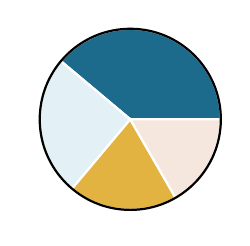
\begin{tikzpicture}\filldraw[fill=accent, draw=white, thick] (0,0) -- (0:1.15) arc (0:140:1.15) -- cycle;\filldraw[fill=accentlight, draw=white, thick] (0,0) -- (140:1.15) arc (140:230:1.15) -- cycle;\filldraw[fill=warmedge, draw=white, thick] (0,0) -- (230:1.15) arc (230:300:1.15) -- cycle;\filldraw[fill=checklight, draw=white, thick] (0,0) -- (300:1.15) arc (300:360:1.15) -- cycle;\draw[thick] (0,0) circle (1.15);\end{tikzpicture}} & \textbf{Pie chart} & \textbf{Categorical} data, to show \textbf{parts of a whole} (fractions or percentages of the total). \\ \hline
\raisebox{-0.5\height}{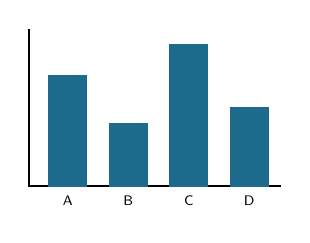
\begin{tikzpicture}[x=0.3200cm,y=0.2000cm]\draw[thick] (0,10) -- (0,0) -- (10,0);\filldraw[fill=accent, draw=accent] (0.8,0) rectangle (2.3,7);\node[below, font=\tiny] at (1.55,0) {A};\filldraw[fill=accent, draw=accent] (3.2,0) rectangle (4.7,4);\node[below, font=\tiny] at (3.95,0) {B};\filldraw[fill=accent, draw=accent] (5.6,0) rectangle (7.1,9);\node[below, font=\tiny] at (6.35,0) {C};\filldraw[fill=accent, draw=accent] (8,0) rectangle (9.5,5);\node[below, font=\tiny] at (8.75,0) {D};\end{tikzpicture}} & \textbf{Bar graph} & \textbf{Categorical} (or discrete) data, to \textbf{compare amounts}. The bars have \textbf{gaps} between them. \\ \hline
\raisebox{-0.5\height}{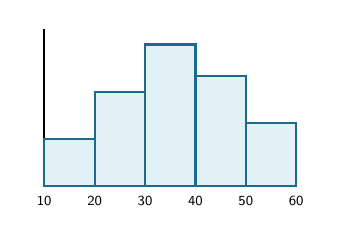
\begin{tikzpicture}[x=0.3200cm,y=0.2000cm]\draw[thick] (0,10) -- (0,0) -- (10,0);\filldraw[fill=accentlight, draw=accent, thick] (0,0) rectangle (2,3);\filldraw[fill=accentlight, draw=accent, thick] (2,0) rectangle (4,6);\filldraw[fill=accentlight, draw=accent, thick] (4,0) rectangle (6,9);\filldraw[fill=accentlight, draw=accent, thick] (6,0) rectangle (8,7);\filldraw[fill=accentlight, draw=accent, thick] (8,0) rectangle (10,4);\node[below, font=\tiny] at (0,0) {10};\node[below, font=\tiny] at (2,0) {20};\node[below, font=\tiny] at (4,0) {30};\node[below, font=\tiny] at (6,0) {40};\node[below, font=\tiny] at (8,0) {50};\node[below, font=\tiny] at (10,0) {60};\end{tikzpicture}} & \textbf{Histogram} & \textbf{Continuous numerical} data in \textbf{groups} (like 150--155\,cm). The bars \textbf{touch} --- no gaps. \\ \hline
\raisebox{-0.5\height}{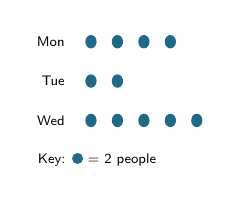
\begin{tikzpicture}[x=0.42cm,y=0.5cm]\node[left, font=\tiny] at (0,0) {Mon};\fill[accent] (0.5,0) circle (0.17);\fill[accent] (1.3,0) circle (0.17);\fill[accent] (2.1,0) circle (0.17);\fill[accent] (2.9,0) circle (0.17);\node[left, font=\tiny] at (0,-1) {Tue};\fill[accent] (0.5,-1) circle (0.17);\fill[accent] (1.3,-1) circle (0.17);\node[left, font=\tiny] at (0,-2) {Wed};\fill[accent] (0.5,-2) circle (0.17);\fill[accent] (1.3,-2) circle (0.17);\fill[accent] (2.1,-2) circle (0.17);\fill[accent] (2.9,-2) circle (0.17);\fill[accent] (3.7,-2) circle (0.17);\node[font=\tiny, anchor=west] at (-1.4,-3) {Key: \tikz\fill[accent] (0,0) circle (0.07cm); = 2 people};\end{tikzpicture}} & \textbf{Pictograph} & \textbf{Categorical} data shown with \textbf{pictures}. There is always a \textbf{key} saying what one picture is worth. \\ \hline
\raisebox{-0.5\height}{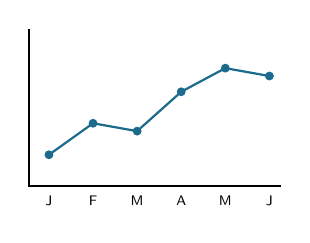
\begin{tikzpicture}[x=0.3200cm,y=0.2000cm]\draw[thick] (0,10) -- (0,0) -- (10,0);\draw[accent, thick] (0.8,2) -- (2.55,4) -- (4.3,3.5) -- (6.05,6) -- (7.8,7.5) -- (9.55,7);\fill[accent] (0.8,2) circle (1.6pt);\fill[accent] (2.55,4) circle (1.6pt);\fill[accent] (4.3,3.5) circle (1.6pt);\fill[accent] (6.05,6) circle (1.6pt);\fill[accent] (7.8,7.5) circle (1.6pt);\fill[accent] (9.55,7) circle (1.6pt);\node[below, font=\tiny] at (0.8,0) {J};\node[below, font=\tiny] at (2.55,0) {F};\node[below, font=\tiny] at (4.3,0) {M};\node[below, font=\tiny] at (6.05,0) {A};\node[below, font=\tiny] at (7.8,0) {M};\node[below, font=\tiny] at (9.55,0) {J};\end{tikzpicture}} & \textbf{Line graph} & Showing how something \textbf{changes over time} (hours, days, months, years). The points are joined. \\ \hline
\end{tabular}
\end{center}

\begin{rememberbox}
\textbf{Bar graph or histogram?} Look at the gaps. Bar graphs have gaps between the bars because each bar is a separate category.
Histograms have \textbf{no gaps} because the groups of numbers follow on from each other.
\end{rememberbox}

\begin{tipbox}{Choosing a display}
Is it about \textbf{time}? Use a line graph. \; Is it \textbf{parts of a whole}? Use a pie chart. \;
Is it \textbf{measured} data in groups? Use a histogram. \; Comparing \textbf{categories}? Use a bar graph or pictograph.
\end{tipbox}

\newpage\normalsize
\banner{2}{Data Displays}{Practice}{accent}
{\large\textbf{Use these words: pie chart, bar graph, histogram, pictograph, line graph.}} {\color{muted}Show your working in each box.}\par\vspace{1mm}
\begin{tcbraster}[raster columns=6, raster column skip=4mm, raster row skip=3mm]
\pbox[raster multicolumn=2]{1}{4.4cm}{\par\centering 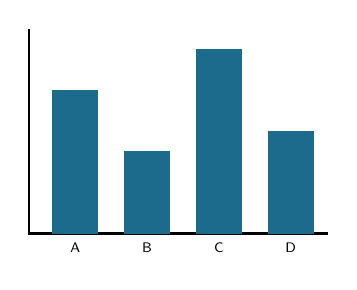
\begin{tikzpicture}[x=0.3800cm,y=0.2600cm]\draw[thick] (0,10) -- (0,0) -- (10,0);\filldraw[fill=accent, draw=accent] (0.8,0) rectangle (2.3,7);\node[below, font=\tiny] at (1.55,0) {A};\filldraw[fill=accent, draw=accent] (3.2,0) rectangle (4.7,4);\node[below, font=\tiny] at (3.95,0) {B};\filldraw[fill=accent, draw=accent] (5.6,0) rectangle (7.1,9);\node[below, font=\tiny] at (6.35,0) {C};\filldraw[fill=accent, draw=accent] (8,0) rectangle (9.5,5);\node[below, font=\tiny] at (8.75,0) {D};\end{tikzpicture}\par\vfill\raggedright This is a\ \ansline{0.6}}
\pbox[raster multicolumn=2]{2}{4.4cm}{\par\centering 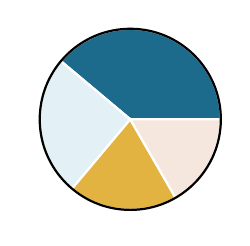
\begin{tikzpicture}\filldraw[fill=accent, draw=white, thick] (0,0) -- (0:1.15) arc (0:140:1.15) -- cycle;\filldraw[fill=accentlight, draw=white, thick] (0,0) -- (140:1.15) arc (140:230:1.15) -- cycle;\filldraw[fill=warmedge, draw=white, thick] (0,0) -- (230:1.15) arc (230:300:1.15) -- cycle;\filldraw[fill=checklight, draw=white, thick] (0,0) -- (300:1.15) arc (300:360:1.15) -- cycle;\draw[thick] (0,0) circle (1.15);\end{tikzpicture}\par\vfill\raggedright This is a\ \ansline{0.6}}
\pbox[raster multicolumn=2]{3}{4.4cm}{\par\centering 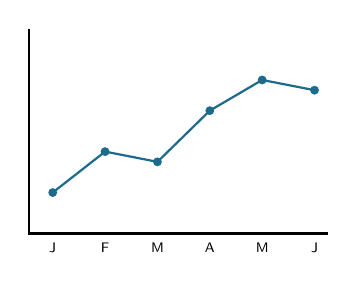
\begin{tikzpicture}[x=0.3800cm,y=0.2600cm]\draw[thick] (0,10) -- (0,0) -- (10,0);\draw[accent, thick] (0.8,2) -- (2.55,4) -- (4.3,3.5) -- (6.05,6) -- (7.8,7.5) -- (9.55,7);\fill[accent] (0.8,2) circle (1.6pt);\fill[accent] (2.55,4) circle (1.6pt);\fill[accent] (4.3,3.5) circle (1.6pt);\fill[accent] (6.05,6) circle (1.6pt);\fill[accent] (7.8,7.5) circle (1.6pt);\fill[accent] (9.55,7) circle (1.6pt);\node[below, font=\tiny] at (0.8,0) {J};\node[below, font=\tiny] at (2.55,0) {F};\node[below, font=\tiny] at (4.3,0) {M};\node[below, font=\tiny] at (6.05,0) {A};\node[below, font=\tiny] at (7.8,0) {M};\node[below, font=\tiny] at (9.55,0) {J};\end{tikzpicture}\par\vfill\raggedright This is a\ \ansline{0.6}}
\pbox[raster multicolumn=2]{4}{4.4cm}{\par\centering 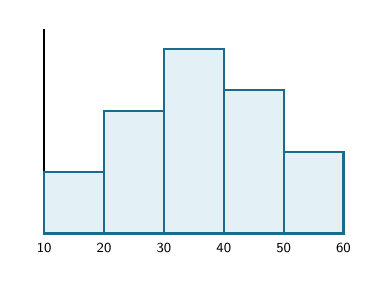
\begin{tikzpicture}[x=0.3800cm,y=0.2600cm]\draw[thick] (0,10) -- (0,0) -- (10,0);\filldraw[fill=accentlight, draw=accent, thick] (0,0) rectangle (2,3);\filldraw[fill=accentlight, draw=accent, thick] (2,0) rectangle (4,6);\filldraw[fill=accentlight, draw=accent, thick] (4,0) rectangle (6,9);\filldraw[fill=accentlight, draw=accent, thick] (6,0) rectangle (8,7);\filldraw[fill=accentlight, draw=accent, thick] (8,0) rectangle (10,4);\node[below, font=\tiny] at (0,0) {10};\node[below, font=\tiny] at (2,0) {20};\node[below, font=\tiny] at (4,0) {30};\node[below, font=\tiny] at (6,0) {40};\node[below, font=\tiny] at (8,0) {50};\node[below, font=\tiny] at (10,0) {60};\end{tikzpicture}\par\vfill\raggedright This is a\ \ansline{0.6}}
\pbox[raster multicolumn=2]{5}{4.4cm}{\par\centering 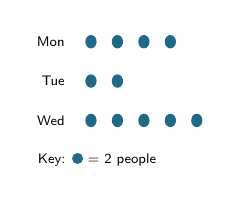
\begin{tikzpicture}[x=0.42cm,y=0.5cm]\node[left, font=\tiny] at (0,0) {Mon};\fill[accent] (0.5,0) circle (0.17);\fill[accent] (1.3,0) circle (0.17);\fill[accent] (2.1,0) circle (0.17);\fill[accent] (2.9,0) circle (0.17);\node[left, font=\tiny] at (0,-1) {Tue};\fill[accent] (0.5,-1) circle (0.17);\fill[accent] (1.3,-1) circle (0.17);\node[left, font=\tiny] at (0,-2) {Wed};\fill[accent] (0.5,-2) circle (0.17);\fill[accent] (1.3,-2) circle (0.17);\fill[accent] (2.1,-2) circle (0.17);\fill[accent] (2.9,-2) circle (0.17);\fill[accent] (3.7,-2) circle (0.17);\node[font=\tiny, anchor=west] at (-1.4,-3) {Key: \tikz\fill[accent] (0,0) circle (0.07cm); = 2 people};\end{tikzpicture}\par\vfill\raggedright This is a\ \ansline{0.6}}
\pbox[raster multicolumn=2]{6}{4.4cm}{\par\centering 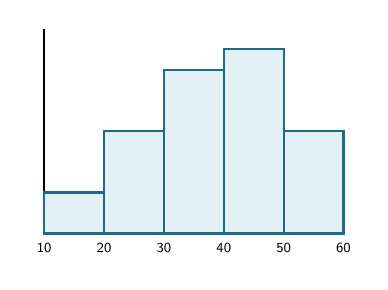
\begin{tikzpicture}[x=0.3800cm,y=0.2600cm]\draw[thick] (0,10) -- (0,0) -- (10,0);\filldraw[fill=accentlight, draw=accent, thick] (0,0) rectangle (2,2);\filldraw[fill=accentlight, draw=accent, thick] (2,0) rectangle (4,5);\filldraw[fill=accentlight, draw=accent, thick] (4,0) rectangle (6,8);\filldraw[fill=accentlight, draw=accent, thick] (6,0) rectangle (8,9);\filldraw[fill=accentlight, draw=accent, thick] (8,0) rectangle (10,5);\node[below, font=\tiny] at (0,0) {10};\node[below, font=\tiny] at (2,0) {20};\node[below, font=\tiny] at (4,0) {30};\node[below, font=\tiny] at (6,0) {40};\node[below, font=\tiny] at (8,0) {50};\node[below, font=\tiny] at (10,0) {60};\end{tikzpicture}\par\vfill\raggedright This is a\ \ansline{0.6}}
\pbox[raster multicolumn=3]{7}{2.9cm}{{\large Best display to show how the temperature changed each hour during a day?}\par\vfill \ansline{0.95}}
\pbox[raster multicolumn=3]{8}{2.9cm}{{\large Best display to show what fraction of the class chose each favourite fruit?}\par\vfill \ansline{0.95}}
\pbox[raster multicolumn=3]{9}{2.9cm}{{\large Best display to compare how many students play rugby, netball, football and hockey?}\par\vfill \ansline{0.95}}
\pbox[raster multicolumn=3]{10}{2.9cm}{{\large Best display for the heights of 30 students, grouped into 150--155\,cm, 155--160\,cm, \ldots?}\par\vfill \ansline{0.95}}
\pbox[raster multicolumn=3]{11}{2.9cm}{{\large Best display to show books read by four friends, using a picture of a book for every 2 books?}\par\vfill \ansline{0.95}}
\pbox[raster multicolumn=3]{12}{2.9cm}{{\large Best display to show a shop's sales each month for a year?}\par\vfill \ansline{0.95}}
\end{tcbraster}
\vfill\centerline{\color{good}\bfseries \ding{51}\ Check your answers at the back. Fix any you got wrong.}
\newpage
\banner{3}{Scatter Plots}{Learn}{accent}
\begin{tcolorbox}[enhanced, colback=accentlight, colframe=accent, boxrule=0pt, leftrule=1.5mm, arc=0mm, top=1.5mm, bottom=1.5mm]\textbf{Goal:} I can describe a point in context, and the strength of a scatter plot\end{tcolorbox}
\large

A \textbf{scatter plot} shows \textbf{two numerical variables} for each person or thing. \textbf{Each dot is one person.}

\begin{minipage}[t]{0.5\linewidth}\vspace{0pt}\hspace*{8mm}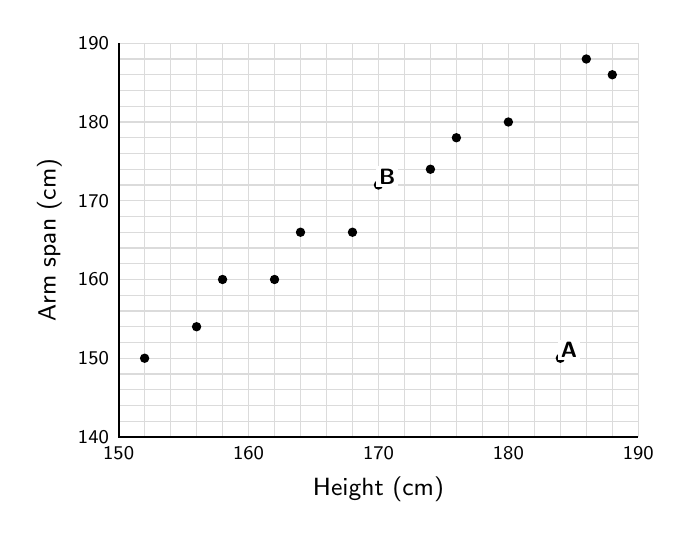
\begin{tikzpicture}[x=0.16500cm,y=0.10000cm, baseline=(current bounding box.north)]\draw[black!14] (0,0) -- (0,50);\node[below, font=\scriptsize] at (0,0) {150};\draw[black!14] (2,0) -- (2,50);\draw[black!14] (4,0) -- (4,50);\draw[black!14] (6,0) -- (6,50);\draw[black!14] (8,0) -- (8,50);\draw[black!14] (10,0) -- (10,50);\node[below, font=\scriptsize] at (10,0) {160};\draw[black!14] (12,0) -- (12,50);\draw[black!14] (14,0) -- (14,50);\draw[black!14] (16,0) -- (16,50);\draw[black!14] (18,0) -- (18,50);\draw[black!14] (20,0) -- (20,50);\node[below, font=\scriptsize] at (20,0) {170};\draw[black!14] (22,0) -- (22,50);\draw[black!14] (24,0) -- (24,50);\draw[black!14] (26,0) -- (26,50);\draw[black!14] (28,0) -- (28,50);\draw[black!14] (30,0) -- (30,50);\node[below, font=\scriptsize] at (30,0) {180};\draw[black!14] (32,0) -- (32,50);\draw[black!14] (34,0) -- (34,50);\draw[black!14] (36,0) -- (36,50);\draw[black!14] (38,0) -- (38,50);\draw[black!14] (40,0) -- (40,50);\node[below, font=\scriptsize] at (40,0) {190};\draw[black!14] (0,0) -- (40,0);\node[left, font=\scriptsize] at (0,0) {140};\draw[black!14] (0,2) -- (40,2);\draw[black!14] (0,4) -- (40,4);\draw[black!14] (0,6) -- (40,6);\draw[black!14] (0,8) -- (40,8);\draw[black!14] (0,10) -- (40,10);\node[left, font=\scriptsize] at (0,10) {150};\draw[black!14] (0,12) -- (40,12);\draw[black!14] (0,14) -- (40,14);\draw[black!14] (0,16) -- (40,16);\draw[black!14] (0,18) -- (40,18);\draw[black!14] (0,20) -- (40,20);\node[left, font=\scriptsize] at (0,20) {160};\draw[black!14] (0,22) -- (40,22);\draw[black!14] (0,24) -- (40,24);\draw[black!14] (0,26) -- (40,26);\draw[black!14] (0,28) -- (40,28);\draw[black!14] (0,30) -- (40,30);\node[left, font=\scriptsize] at (0,30) {170};\draw[black!14] (0,32) -- (40,32);\draw[black!14] (0,34) -- (40,34);\draw[black!14] (0,36) -- (40,36);\draw[black!14] (0,38) -- (40,38);\draw[black!14] (0,40) -- (40,40);\node[left, font=\scriptsize] at (0,40) {180};\draw[black!14] (0,42) -- (40,42);\draw[black!14] (0,44) -- (40,44);\draw[black!14] (0,46) -- (40,46);\draw[black!14] (0,48) -- (40,48);\draw[black!14] (0,50) -- (40,50);\node[left, font=\scriptsize] at (0,50) {190};\draw[thick] (0,50) -- (0,0) -- (40,0);\node[below=11pt, font=\small] at (20,0) {Height (cm)};\node[rotate=90, above=17pt, font=\small] at (0,25) {Arm span (cm)};\fill (2,10) circle (1.7pt);\fill (6,14) circle (1.7pt);\fill (8,20) circle (1.7pt);\fill (12,20) circle (1.7pt);\fill (14,26) circle (1.7pt);\fill (18,26) circle (1.7pt);\fill (20,32) circle (1.7pt);\fill (24,34) circle (1.7pt);\fill (26,38) circle (1.7pt);\fill (30,40) circle (1.7pt);\fill (34,10) circle (1.7pt);\fill (36,48) circle (1.7pt);\fill (38,46) circle (1.7pt);\node[above right=-1pt, font=\footnotesize\bfseries, fill=white, inner sep=1pt] at (34,10) {A};\node[above right=-1pt, font=\footnotesize\bfseries, fill=white, inner sep=1pt] at (20,32) {B};\end{tikzpicture}\end{minipage}\hfill
\begin{minipage}[t]{0.46\linewidth}\vspace{0pt}
\textbf{Describing a point in context}\\[2pt]
Read \textbf{down} to the bottom axis and \textbf{across} to the side axis. Then write a sentence that uses
\textbf{both} variables and their \textbf{units}.\\[6pt]
\textbf{Point A} is a person who is 184\,cm tall and has an arm span of 150\,cm.\\[6pt]
\textbf{Point B} is a person who is 170\,cm tall and has an arm span of 172\,cm.\\[6pt]
Point A is \textbf{unusual}: it doesn't follow the pattern of the other points.
\end{minipage}

\vspace{9mm}
\subsection*{Describing the relationship}
\textbf{Direction:} \textbf{positive} if the points go \textbf{uphill} (as one goes up, the other goes up);
\textbf{negative} if they go \textbf{downhill}.\\
\textbf{Strength:} how closely the points follow a straight line.

\begin{center}
\begin{tabular}{cccc}
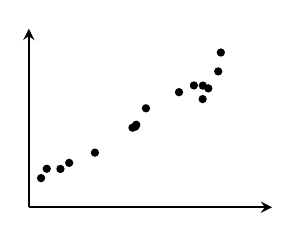
\begin{tikzpicture}[x=0.3000cm,y=0.2200cm]\draw[thick,->,>=stealth] (0,0) -- (10.3,0); \draw[thick,->,>=stealth] (0,0) -- (0,10.3);\fill (1.71,2.56) circle (1.5pt);\fill (8.13,8.93) circle (1.5pt);\fill (7.37,7.02) circle (1.5pt);\fill (2.80,3.15) circle (1.5pt);\fill (4.96,5.71) circle (1.5pt);\fill (4.55,4.76) circle (1.5pt);\fill (6.36,6.64) circle (1.5pt);\fill (7.60,6.86) circle (1.5pt);\fill (1.34,2.21) circle (1.5pt);\fill (0.76,2.22) circle (1.5pt);\fill (8.02,7.84) circle (1.5pt);\fill (4.39,4.59) circle (1.5pt);\fill (7.36,6.24) circle (1.5pt);\fill (0.52,1.68) circle (1.5pt);\fill (4.51,4.65) circle (1.5pt);\fill (6.99,7.03) circle (1.5pt);\end{tikzpicture} & 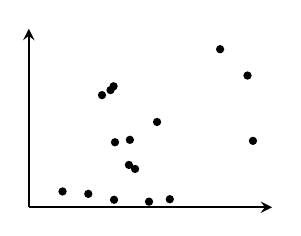
\begin{tikzpicture}[x=0.3000cm,y=0.2200cm]\draw[thick,->,>=stealth] (0,0) -- (10.3,0); \draw[thick,->,>=stealth] (0,0) -- (0,10.3);\fill (5.43,4.92) circle (1.5pt);\fill (3.61,0.43) circle (1.5pt);\fill (8.10,9.12) circle (1.5pt);\fill (3.10,6.47) circle (1.5pt);\fill (5.09,0.32) circle (1.5pt);\fill (3.59,6.98) circle (1.5pt);\fill (4.24,2.44) circle (1.5pt);\fill (9.26,7.60) circle (1.5pt);\fill (1.43,0.91) circle (1.5pt);\fill (4.50,2.21) circle (1.5pt);\fill (2.52,0.77) circle (1.5pt);\fill (3.65,3.75) circle (1.5pt);\fill (9.49,3.83) circle (1.5pt);\fill (3.46,6.76) circle (1.5pt);\fill (5.97,0.46) circle (1.5pt);\fill (4.28,3.89) circle (1.5pt);\end{tikzpicture} & 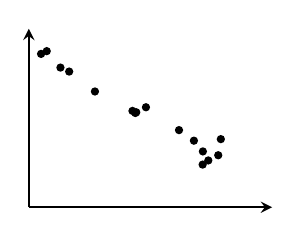
\begin{tikzpicture}[x=0.3000cm,y=0.2200cm]\draw[thick,->,>=stealth] (0,0) -- (10.3,0); \draw[thick,->,>=stealth] (0,0) -- (0,10.3);\fill (1.71,7.83) circle (1.5pt);\fill (8.13,3.93) circle (1.5pt);\fill (7.37,3.22) circle (1.5pt);\fill (2.80,6.68) circle (1.5pt);\fill (4.96,5.77) circle (1.5pt);\fill (4.55,5.48) circle (1.5pt);\fill (6.36,4.45) circle (1.5pt);\fill (7.60,2.70) circle (1.5pt);\fill (1.34,8.06) circle (1.5pt);\fill (0.76,9.01) circle (1.5pt);\fill (8.02,3.00) circle (1.5pt);\fill (4.39,5.56) circle (1.5pt);\fill (7.36,2.46) circle (1.5pt);\fill (0.52,8.85) circle (1.5pt);\fill (4.51,5.44) circle (1.5pt);\fill (6.99,3.84) circle (1.5pt);\end{tikzpicture} & 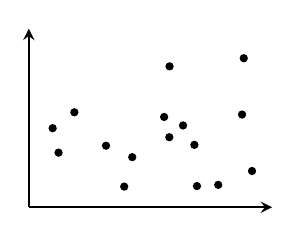
\begin{tikzpicture}[x=0.3000cm,y=0.2200cm]\draw[thick,->,>=stealth] (0,0) -- (10.3,0); \draw[thick,->,>=stealth] (0,0) -- (0,10.3);\fill (9.10,8.60) circle (1.5pt);\fill (9.03,5.35) circle (1.5pt);\fill (1.01,4.56) circle (1.5pt);\fill (1.26,3.15) circle (1.5pt);\fill (8.02,1.29) circle (1.5pt);\fill (7.12,1.22) circle (1.5pt);\fill (6.53,4.72) circle (1.5pt);\fill (3.27,3.55) circle (1.5pt);\fill (5.95,4.04) circle (1.5pt);\fill (5.96,8.13) circle (1.5pt);\fill (5.73,5.21) circle (1.5pt);\fill (1.93,5.48) circle (1.5pt);\fill (4.38,2.89) circle (1.5pt);\fill (4.04,1.19) circle (1.5pt);\fill (7.01,3.60) circle (1.5pt);\fill (9.45,2.09) circle (1.5pt);\end{tikzpicture} \\
\textbf{Strong positive} & \textbf{Weak positive} & \textbf{Strong negative} & \textbf{No relationship} \\
{\small Close to a line} & {\small Spread out, slight trend} & {\small Close to a line} & {\small No pattern}
\end{tabular}
\end{center}

\begin{rememberbox}
\textbf{Strong}: the points are close to a straight line. \textbf{Moderate}: they follow a line but are more spread out.
\textbf{Weak}: there is only a slight trend. Always give the \textbf{strength} and the \textbf{direction}, e.g. \textquotedblleft{}moderate positive\textquotedblright{}.
\end{rememberbox}

\newpage\normalsize
\banner{3}{Scatter Plots}{Practice}{accent}
{\large\textbf{Answer (a)--(e) using the scatter plot. Then describe each small scatter plot.}} {\color{muted}Show your working in each box.}\par\vspace{1mm}
\begin{tcbraster}[raster columns=6, raster column skip=4mm, raster row skip=3mm]
\pbox[raster multicolumn=6]{1}{10.8cm}{\textbf{Hours of study and test score for 13 students}\par\vspace{1mm}\begin{minipage}[t]{0.52\linewidth}\vspace{0pt}\hspace*{9mm}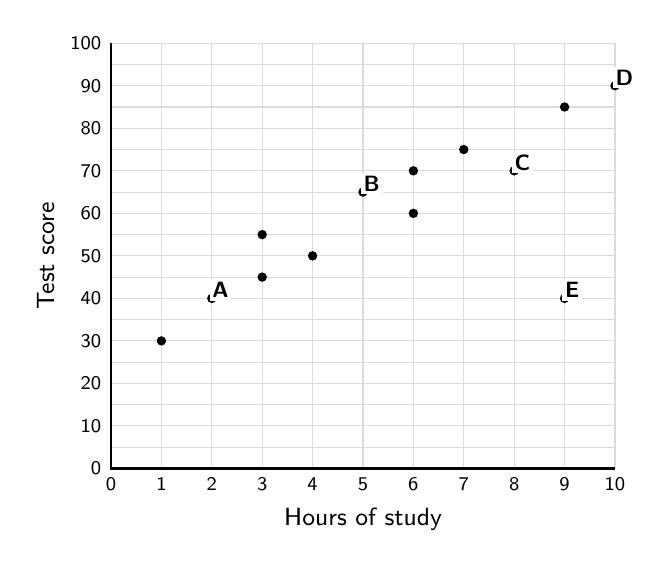
\begin{tikzpicture}[x=0.64000cm,y=0.05400cm, baseline=(current bounding box.north)]\draw[black!14] (0,0) -- (0,100);\node[below, font=\scriptsize] at (0,0) {0};\draw[black!14] (1,0) -- (1,100);\node[below, font=\scriptsize] at (1,0) {1};\draw[black!14] (2,0) -- (2,100);\node[below, font=\scriptsize] at (2,0) {2};\draw[black!14] (3,0) -- (3,100);\node[below, font=\scriptsize] at (3,0) {3};\draw[black!14] (4,0) -- (4,100);\node[below, font=\scriptsize] at (4,0) {4};\draw[black!14] (5,0) -- (5,100);\node[below, font=\scriptsize] at (5,0) {5};\draw[black!14] (6,0) -- (6,100);\node[below, font=\scriptsize] at (6,0) {6};\draw[black!14] (7,0) -- (7,100);\node[below, font=\scriptsize] at (7,0) {7};\draw[black!14] (8,0) -- (8,100);\node[below, font=\scriptsize] at (8,0) {8};\draw[black!14] (9,0) -- (9,100);\node[below, font=\scriptsize] at (9,0) {9};\draw[black!14] (10,0) -- (10,100);\node[below, font=\scriptsize] at (10,0) {10};\draw[black!14] (0,0) -- (10,0);\node[left, font=\scriptsize] at (0,0) {0};\draw[black!14] (0,5) -- (10,5);\draw[black!14] (0,10) -- (10,10);\node[left, font=\scriptsize] at (0,10) {10};\draw[black!14] (0,15) -- (10,15);\draw[black!14] (0,20) -- (10,20);\node[left, font=\scriptsize] at (0,20) {20};\draw[black!14] (0,25) -- (10,25);\draw[black!14] (0,30) -- (10,30);\node[left, font=\scriptsize] at (0,30) {30};\draw[black!14] (0,35) -- (10,35);\draw[black!14] (0,40) -- (10,40);\node[left, font=\scriptsize] at (0,40) {40};\draw[black!14] (0,45) -- (10,45);\draw[black!14] (0,50) -- (10,50);\node[left, font=\scriptsize] at (0,50) {50};\draw[black!14] (0,55) -- (10,55);\draw[black!14] (0,60) -- (10,60);\node[left, font=\scriptsize] at (0,60) {60};\draw[black!14] (0,65) -- (10,65);\draw[black!14] (0,70) -- (10,70);\node[left, font=\scriptsize] at (0,70) {70};\draw[black!14] (0,75) -- (10,75);\draw[black!14] (0,80) -- (10,80);\node[left, font=\scriptsize] at (0,80) {80};\draw[black!14] (0,85) -- (10,85);\draw[black!14] (0,90) -- (10,90);\node[left, font=\scriptsize] at (0,90) {90};\draw[black!14] (0,95) -- (10,95);\draw[black!14] (0,100) -- (10,100);\node[left, font=\scriptsize] at (0,100) {100};\draw[thick] (0,100) -- (0,0) -- (10,0);\node[below=11pt, font=\small] at (5,0) {Hours of study};\node[rotate=90, above=17pt, font=\small] at (0,50) {Test score};\fill (1,30) circle (1.7pt);\fill (2,40) circle (1.7pt);\fill (3,45) circle (1.7pt);\fill (3,55) circle (1.7pt);\fill (4,50) circle (1.7pt);\fill (5,65) circle (1.7pt);\fill (6,60) circle (1.7pt);\fill (6,70) circle (1.7pt);\fill (7,75) circle (1.7pt);\fill (8,70) circle (1.7pt);\fill (9,85) circle (1.7pt);\fill (10,90) circle (1.7pt);\fill (9,40) circle (1.7pt);\node[above right=-1pt, font=\footnotesize\bfseries, fill=white, inner sep=1pt] at (2,40) {A};\node[above right=-1pt, font=\footnotesize\bfseries, fill=white, inner sep=1pt] at (5,65) {B};\node[above right=-1pt, font=\footnotesize\bfseries, fill=white, inner sep=1pt] at (8,70) {C};\node[above right=-1pt, font=\footnotesize\bfseries, fill=white, inner sep=1pt] at (10,90) {D};\node[above right=-1pt, font=\footnotesize\bfseries, fill=white, inner sep=1pt] at (9,40) {E};\end{tikzpicture}\end{minipage}\hfill\begin{minipage}[t]{0.46\linewidth}\vspace{0pt}{\small\textbf{(a)} Describe point \textbf{A} in context.}\par\vspace{4mm}\ansline{1}\par\vspace{3mm}{\small\textbf{(b)} Describe point \textbf{B} in context.}\par\vspace{4mm}\ansline{1}\par\vspace{3mm}{\small\textbf{(c)} Describe point \textbf{E} in context.}\par\vspace{4mm}\ansline{1}\par\vspace{3mm}{\small\textbf{(d)} Which point is a student who studied for 10 hours and scored 90 marks?}\par\vspace{4mm}\ansline{1}\par\vspace{3mm}{\small\textbf{(e)} Describe the strength and direction of the relationship.}\par\vspace{4mm}\ansline{1}\end{minipage}}
\pbox[raster multicolumn=2]{2}{4.3cm}{\par\centering 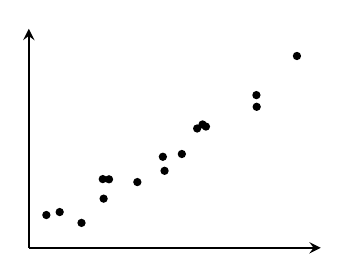
\begin{tikzpicture}[x=0.3600cm,y=0.2700cm]\draw[thick,->,>=stealth] (0,0) -- (10.3,0); \draw[thick,->,>=stealth] (0,0) -- (0,10.3);\fill (2.64,2.31) circle (1.5pt);\fill (5.40,4.41) circle (1.5pt);\fill (3.83,3.09) circle (1.5pt);\fill (5.94,5.61) circle (1.5pt);\fill (6.13,5.80) circle (1.5pt);\fill (1.09,1.68) circle (1.5pt);\fill (0.62,1.54) circle (1.5pt);\fill (8.04,6.63) circle (1.5pt);\fill (2.83,3.22) circle (1.5pt);\fill (2.61,3.23) circle (1.5pt);\fill (9.46,9.02) circle (1.5pt);\fill (4.73,4.28) circle (1.5pt);\fill (8.03,7.18) circle (1.5pt);\fill (4.79,3.62) circle (1.5pt);\fill (6.25,5.70) circle (1.5pt);\fill (1.86,1.17) circle (1.5pt);\end{tikzpicture}\par\vfill\raggedright\ansline{0.95}}
\pbox[raster multicolumn=2]{3}{4.3cm}{\par\centering 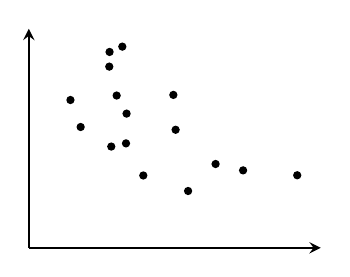
\begin{tikzpicture}[x=0.3600cm,y=0.2700cm]\draw[thick,->,>=stealth] (0,0) -- (10.3,0); \draw[thick,->,>=stealth] (0,0) -- (0,10.3);\fill (6.59,3.94) circle (1.5pt);\fill (7.56,3.64) circle (1.5pt);\fill (5.18,5.55) circle (1.5pt);\fill (5.10,7.19) circle (1.5pt);\fill (4.04,3.40) circle (1.5pt);\fill (9.47,3.41) circle (1.5pt);\fill (3.10,7.16) circle (1.5pt);\fill (1.83,5.68) circle (1.5pt);\fill (2.85,9.21) circle (1.5pt);\fill (2.84,8.52) circle (1.5pt);\fill (3.45,6.31) circle (1.5pt);\fill (2.91,4.76) circle (1.5pt);\fill (1.47,6.95) circle (1.5pt);\fill (3.43,4.91) circle (1.5pt);\fill (3.30,9.46) circle (1.5pt);\fill (5.62,2.67) circle (1.5pt);\end{tikzpicture}\par\vfill\raggedright\ansline{0.95}}
\pbox[raster multicolumn=2]{4}{4.3cm}{\par\centering 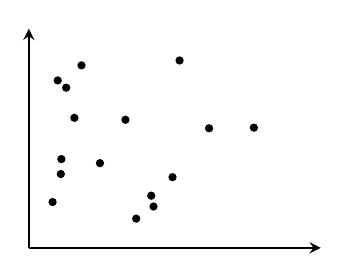
\begin{tikzpicture}[x=0.3600cm,y=0.2700cm]\draw[thick,->,>=stealth] (0,0) -- (10.3,0); \draw[thick,->,>=stealth] (0,0) -- (0,10.3);\fill (3.41,6.02) circle (1.5pt);\fill (1.86,8.58) circle (1.5pt);\fill (6.36,5.62) circle (1.5pt);\fill (1.15,4.17) circle (1.5pt);\fill (5.32,8.81) circle (1.5pt);\fill (3.79,1.37) circle (1.5pt);\fill (1.02,7.87) circle (1.5pt);\fill (5.07,3.32) circle (1.5pt);\fill (0.84,2.15) circle (1.5pt);\fill (4.40,1.94) circle (1.5pt);\fill (1.13,3.47) circle (1.5pt);\fill (1.32,7.53) circle (1.5pt);\fill (4.32,2.45) circle (1.5pt);\fill (7.94,5.65) circle (1.5pt);\fill (1.61,6.11) circle (1.5pt);\fill (2.51,3.98) circle (1.5pt);\end{tikzpicture}\par\vfill\raggedright\ansline{0.95}}
\pbox[raster multicolumn=2]{5}{4.3cm}{\par\centering 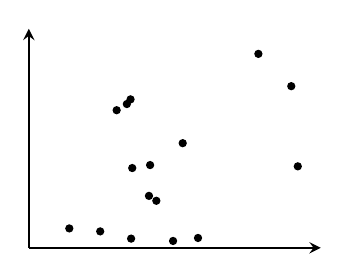
\begin{tikzpicture}[x=0.3600cm,y=0.2700cm]\draw[thick,->,>=stealth] (0,0) -- (10.3,0); \draw[thick,->,>=stealth] (0,0) -- (0,10.3);\fill (5.43,4.92) circle (1.5pt);\fill (3.61,0.43) circle (1.5pt);\fill (8.10,9.12) circle (1.5pt);\fill (3.10,6.47) circle (1.5pt);\fill (5.09,0.32) circle (1.5pt);\fill (3.59,6.98) circle (1.5pt);\fill (4.24,2.44) circle (1.5pt);\fill (9.26,7.60) circle (1.5pt);\fill (1.43,0.91) circle (1.5pt);\fill (4.50,2.21) circle (1.5pt);\fill (2.52,0.77) circle (1.5pt);\fill (3.65,3.75) circle (1.5pt);\fill (9.49,3.83) circle (1.5pt);\fill (3.46,6.76) circle (1.5pt);\fill (5.97,0.46) circle (1.5pt);\fill (4.28,3.89) circle (1.5pt);\end{tikzpicture}\par\vfill\raggedright\ansline{0.95}}
\pbox[raster multicolumn=2]{6}{4.3cm}{\par\centering 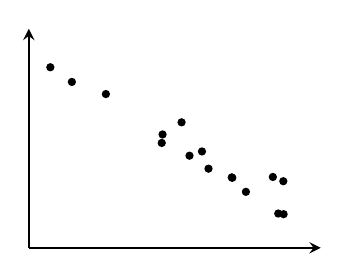
\begin{tikzpicture}[x=0.3600cm,y=0.2700cm]\draw[thick,->,>=stealth] (0,0) -- (10.3,0); \draw[thick,->,>=stealth] (0,0) -- (0,10.3);\fill (6.11,4.53) circle (1.5pt);\fill (7.18,3.29) circle (1.5pt);\fill (7.66,2.63) circle (1.5pt);\fill (8.98,3.13) circle (1.5pt);\fill (7.16,3.31) circle (1.5pt);\fill (8.80,1.61) circle (1.5pt);\fill (0.76,8.49) circle (1.5pt);\fill (4.69,4.93) circle (1.5pt);\fill (8.99,1.58) circle (1.5pt);\fill (6.34,3.72) circle (1.5pt);\fill (8.61,3.33) circle (1.5pt);\fill (1.52,7.80) circle (1.5pt);\fill (4.72,5.33) circle (1.5pt);\fill (2.72,7.23) circle (1.5pt);\fill (5.39,5.90) circle (1.5pt);\fill (5.67,4.33) circle (1.5pt);\end{tikzpicture}\par\vfill\raggedright\ansline{0.95}}
\pbox[raster multicolumn=2]{7}{4.3cm}{\par\centering 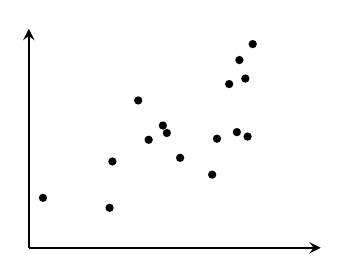
\begin{tikzpicture}[x=0.3600cm,y=0.2700cm]\draw[thick,->,>=stealth] (0,0) -- (10.3,0); \draw[thick,->,>=stealth] (0,0) -- (0,10.3);\fill (7.64,7.96) circle (1.5pt);\fill (7.90,9.58) circle (1.5pt);\fill (4.87,5.40) circle (1.5pt);\fill (2.85,1.88) circle (1.5pt);\fill (0.50,2.35) circle (1.5pt);\fill (6.47,3.44) circle (1.5pt);\fill (4.73,5.75) circle (1.5pt);\fill (7.34,5.44) circle (1.5pt);\fill (3.86,6.93) circle (1.5pt);\fill (7.43,8.83) circle (1.5pt);\fill (2.95,4.06) circle (1.5pt);\fill (7.72,5.23) circle (1.5pt);\fill (7.07,7.70) circle (1.5pt);\fill (4.23,5.08) circle (1.5pt);\fill (5.34,4.23) circle (1.5pt);\fill (6.64,5.13) circle (1.5pt);\end{tikzpicture}\par\vfill\raggedright\ansline{0.95}}
\end{tcbraster}
\vfill\centerline{\color{good}\bfseries \ding{51}\ Check your answers at the back. Fix any you got wrong.}
\newpage
\banner{4}{Lines of Best Fit}{Learn}{accent}
\begin{tcolorbox}[enhanced, colback=accentlight, colframe=accent, boxrule=0pt, leftrule=1.5mm, arc=0mm, top=1.5mm, bottom=1.5mm]\textbf{Goal:} I can draw a line of best fit and use it to make a prediction\end{tcolorbox}
\large

A \textbf{line of best fit} is a straight line that shows the \textbf{trend} of the points.

\begin{stepsbox}{Drawing a line of best fit}
\begin{enumerate}[nosep]
\item Use a \textbf{ruler}. It must be a \textbf{straight} line.
\item Follow the \textbf{direction} of the points, through the \textbf{middle} of them.
\item Have about the \textbf{same number of points above and below} the line.
\item It does \textbf{not} have to go through (0,\,0), or through any particular point.
\end{enumerate}
\end{stepsbox}

\begin{minipage}[t]{0.5\linewidth}\vspace{0pt}\hspace*{8mm}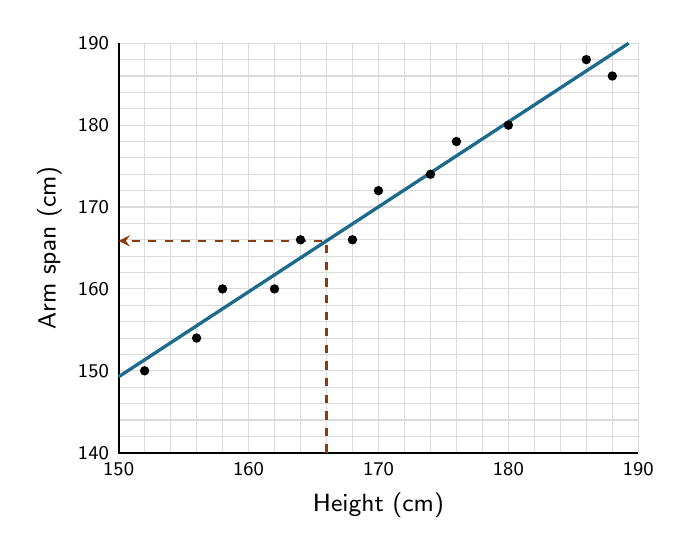
\begin{tikzpicture}[x=0.16500cm,y=0.10400cm, baseline=(current bounding box.north)]\draw[black!14] (0,0) -- (0,50);\node[below, font=\scriptsize] at (0,0) {150};\draw[black!14] (2,0) -- (2,50);\draw[black!14] (4,0) -- (4,50);\draw[black!14] (6,0) -- (6,50);\draw[black!14] (8,0) -- (8,50);\draw[black!14] (10,0) -- (10,50);\node[below, font=\scriptsize] at (10,0) {160};\draw[black!14] (12,0) -- (12,50);\draw[black!14] (14,0) -- (14,50);\draw[black!14] (16,0) -- (16,50);\draw[black!14] (18,0) -- (18,50);\draw[black!14] (20,0) -- (20,50);\node[below, font=\scriptsize] at (20,0) {170};\draw[black!14] (22,0) -- (22,50);\draw[black!14] (24,0) -- (24,50);\draw[black!14] (26,0) -- (26,50);\draw[black!14] (28,0) -- (28,50);\draw[black!14] (30,0) -- (30,50);\node[below, font=\scriptsize] at (30,0) {180};\draw[black!14] (32,0) -- (32,50);\draw[black!14] (34,0) -- (34,50);\draw[black!14] (36,0) -- (36,50);\draw[black!14] (38,0) -- (38,50);\draw[black!14] (40,0) -- (40,50);\node[below, font=\scriptsize] at (40,0) {190};\draw[black!14] (0,0) -- (40,0);\node[left, font=\scriptsize] at (0,0) {140};\draw[black!14] (0,2) -- (40,2);\draw[black!14] (0,4) -- (40,4);\draw[black!14] (0,6) -- (40,6);\draw[black!14] (0,8) -- (40,8);\draw[black!14] (0,10) -- (40,10);\node[left, font=\scriptsize] at (0,10) {150};\draw[black!14] (0,12) -- (40,12);\draw[black!14] (0,14) -- (40,14);\draw[black!14] (0,16) -- (40,16);\draw[black!14] (0,18) -- (40,18);\draw[black!14] (0,20) -- (40,20);\node[left, font=\scriptsize] at (0,20) {160};\draw[black!14] (0,22) -- (40,22);\draw[black!14] (0,24) -- (40,24);\draw[black!14] (0,26) -- (40,26);\draw[black!14] (0,28) -- (40,28);\draw[black!14] (0,30) -- (40,30);\node[left, font=\scriptsize] at (0,30) {170};\draw[black!14] (0,32) -- (40,32);\draw[black!14] (0,34) -- (40,34);\draw[black!14] (0,36) -- (40,36);\draw[black!14] (0,38) -- (40,38);\draw[black!14] (0,40) -- (40,40);\node[left, font=\scriptsize] at (0,40) {180};\draw[black!14] (0,42) -- (40,42);\draw[black!14] (0,44) -- (40,44);\draw[black!14] (0,46) -- (40,46);\draw[black!14] (0,48) -- (40,48);\draw[black!14] (0,50) -- (40,50);\node[left, font=\scriptsize] at (0,50) {190};\draw[thick] (0,50) -- (0,0) -- (40,0);\node[below=11pt, font=\small] at (20,0) {Height (cm)};\node[rotate=90, above=17pt, font=\small] at (0,25) {Arm span (cm)};\draw[accent, very thick] (0,9.27054) -- (39.2608,50);\draw[checkcol, thick, dashed, ->, >=stealth] (16,0) -- (16,25.8691) -- (0,25.8691);\fill (2,10) circle (1.7pt);\fill (6,14) circle (1.7pt);\fill (8,20) circle (1.7pt);\fill (12,20) circle (1.7pt);\fill (14,26) circle (1.7pt);\fill (18,26) circle (1.7pt);\fill (20,32) circle (1.7pt);\fill (24,34) circle (1.7pt);\fill (26,38) circle (1.7pt);\fill (30,40) circle (1.7pt);\fill (36,48) circle (1.7pt);\fill (38,46) circle (1.7pt);\end{tikzpicture}\end{minipage}\hfill
\begin{minipage}[t]{0.46\linewidth}\vspace{0pt}
\textbf{Making a prediction}\\[2pt]
Predict the arm span of a person who is \textbf{166\,cm} tall:
\begin{enumerate}[nosep]
\item Find 166 on the \textbf{bottom} axis.
\item Go \textbf{up} to your line.
\item Go \textbf{across} to the side axis and read the value.
\end{enumerate}
\vspace{3pt}
\textbf{Answer:} about \textbf{166\,cm}.\\[6pt]
To go the other way (from the side axis), go \textbf{across} to the line, then \textbf{down}.
\end{minipage}

\vspace{10mm}
\begin{rememberbox}
A prediction is an \textbf{estimate}, so say \textquotedblleft{}\textbf{about} 166\,cm\textquotedblright{}. Everyone's line is a little different,
so answers close to each other are all fine. Predictions are most reliable \textbf{inside} the range of the data.
\end{rememberbox}

\newpage\normalsize
\banner{4}{Lines of Best Fit}{Practice}{accent}
{\large\textbf{Use a ruler to draw a line of best fit. Then use your line to make the predictions.}} {\color{muted}Show your working in each box.}\par\vspace{1mm}
\begin{tcbraster}[raster columns=2, raster column skip=4mm, raster row skip=3mm]
\pbox[raster multicolumn=2]{1}{9.6cm}{\textbf{Age and value of 14 cars}\par\vspace{1mm}\begin{minipage}[t]{0.52\linewidth}\vspace{0pt}\hspace*{9mm}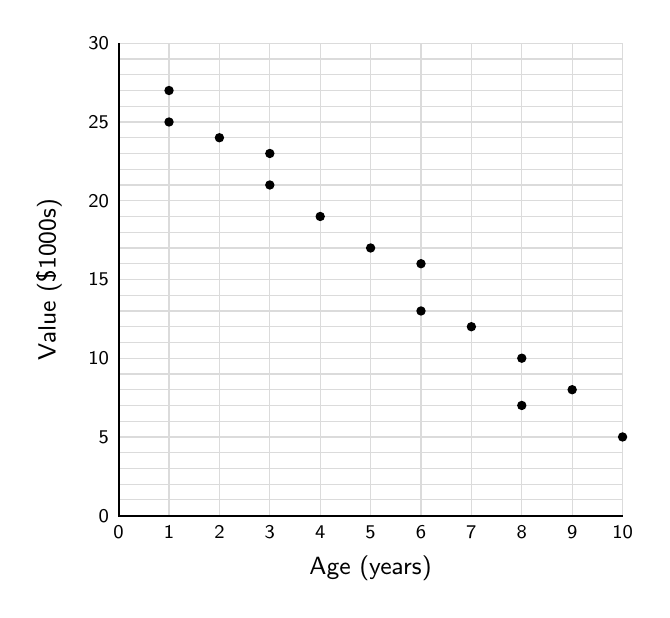
\begin{tikzpicture}[x=0.64000cm,y=0.20000cm, baseline=(current bounding box.north)]\draw[black!14] (0,0) -- (0,30);\node[below, font=\scriptsize] at (0,0) {0};\draw[black!14] (1,0) -- (1,30);\node[below, font=\scriptsize] at (1,0) {1};\draw[black!14] (2,0) -- (2,30);\node[below, font=\scriptsize] at (2,0) {2};\draw[black!14] (3,0) -- (3,30);\node[below, font=\scriptsize] at (3,0) {3};\draw[black!14] (4,0) -- (4,30);\node[below, font=\scriptsize] at (4,0) {4};\draw[black!14] (5,0) -- (5,30);\node[below, font=\scriptsize] at (5,0) {5};\draw[black!14] (6,0) -- (6,30);\node[below, font=\scriptsize] at (6,0) {6};\draw[black!14] (7,0) -- (7,30);\node[below, font=\scriptsize] at (7,0) {7};\draw[black!14] (8,0) -- (8,30);\node[below, font=\scriptsize] at (8,0) {8};\draw[black!14] (9,0) -- (9,30);\node[below, font=\scriptsize] at (9,0) {9};\draw[black!14] (10,0) -- (10,30);\node[below, font=\scriptsize] at (10,0) {10};\draw[black!14] (0,0) -- (10,0);\node[left, font=\scriptsize] at (0,0) {0};\draw[black!14] (0,1) -- (10,1);\draw[black!14] (0,2) -- (10,2);\draw[black!14] (0,3) -- (10,3);\draw[black!14] (0,4) -- (10,4);\draw[black!14] (0,5) -- (10,5);\node[left, font=\scriptsize] at (0,5) {5};\draw[black!14] (0,6) -- (10,6);\draw[black!14] (0,7) -- (10,7);\draw[black!14] (0,8) -- (10,8);\draw[black!14] (0,9) -- (10,9);\draw[black!14] (0,10) -- (10,10);\node[left, font=\scriptsize] at (0,10) {10};\draw[black!14] (0,11) -- (10,11);\draw[black!14] (0,12) -- (10,12);\draw[black!14] (0,13) -- (10,13);\draw[black!14] (0,14) -- (10,14);\draw[black!14] (0,15) -- (10,15);\node[left, font=\scriptsize] at (0,15) {15};\draw[black!14] (0,16) -- (10,16);\draw[black!14] (0,17) -- (10,17);\draw[black!14] (0,18) -- (10,18);\draw[black!14] (0,19) -- (10,19);\draw[black!14] (0,20) -- (10,20);\node[left, font=\scriptsize] at (0,20) {20};\draw[black!14] (0,21) -- (10,21);\draw[black!14] (0,22) -- (10,22);\draw[black!14] (0,23) -- (10,23);\draw[black!14] (0,24) -- (10,24);\draw[black!14] (0,25) -- (10,25);\node[left, font=\scriptsize] at (0,25) {25};\draw[black!14] (0,26) -- (10,26);\draw[black!14] (0,27) -- (10,27);\draw[black!14] (0,28) -- (10,28);\draw[black!14] (0,29) -- (10,29);\draw[black!14] (0,30) -- (10,30);\node[left, font=\scriptsize] at (0,30) {30};\draw[thick] (0,30) -- (0,0) -- (10,0);\node[below=11pt, font=\small] at (5,0) {Age (years)};\node[rotate=90, above=17pt, font=\small] at (0,15) {Value (\$1000s)};\fill (1,27) circle (1.7pt);\fill (1,25) circle (1.7pt);\fill (2,24) circle (1.7pt);\fill (3,21) circle (1.7pt);\fill (3,23) circle (1.7pt);\fill (4,19) circle (1.7pt);\fill (5,17) circle (1.7pt);\fill (6,16) circle (1.7pt);\fill (6,13) circle (1.7pt);\fill (7,12) circle (1.7pt);\fill (8,10) circle (1.7pt);\fill (9,8) circle (1.7pt);\fill (10,5) circle (1.7pt);\fill (8,7) circle (1.7pt);\end{tikzpicture}\end{minipage}\hfill\begin{minipage}[t]{0.46\linewidth}\vspace{0pt}{\small\textbf{(a)} Draw a line of best fit on the graph.}\par\vspace{3mm}{\small\textbf{(b)} Predict the value of a car that is 2 years old.}\par\vspace{4mm}\ansline{1}\par\vspace{3mm}{\small\textbf{(c)} Predict the value of a car that is 7 years old.}\par\vspace{4mm}\ansline{1}\par\vspace{3mm}{\small\textbf{(d)} Predict the age of a car that is worth \$15\,000.}\par\vspace{4mm}\ansline{1}\end{minipage}}
\pbox[raster multicolumn=2]{2}{9.6cm}{\textbf{Temperature and ice creams sold on 13 days}\par\vspace{1mm}\begin{minipage}[t]{0.52\linewidth}\vspace{0pt}\hspace*{9mm}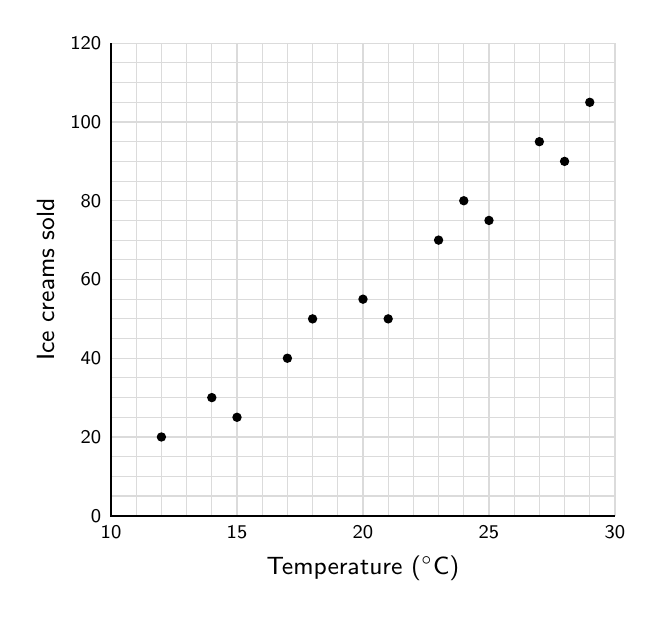
\begin{tikzpicture}[x=0.32000cm,y=0.05000cm, baseline=(current bounding box.north)]\draw[black!14] (0,0) -- (0,120);\node[below, font=\scriptsize] at (0,0) {10};\draw[black!14] (1,0) -- (1,120);\draw[black!14] (2,0) -- (2,120);\draw[black!14] (3,0) -- (3,120);\draw[black!14] (4,0) -- (4,120);\draw[black!14] (5,0) -- (5,120);\node[below, font=\scriptsize] at (5,0) {15};\draw[black!14] (6,0) -- (6,120);\draw[black!14] (7,0) -- (7,120);\draw[black!14] (8,0) -- (8,120);\draw[black!14] (9,0) -- (9,120);\draw[black!14] (10,0) -- (10,120);\node[below, font=\scriptsize] at (10,0) {20};\draw[black!14] (11,0) -- (11,120);\draw[black!14] (12,0) -- (12,120);\draw[black!14] (13,0) -- (13,120);\draw[black!14] (14,0) -- (14,120);\draw[black!14] (15,0) -- (15,120);\node[below, font=\scriptsize] at (15,0) {25};\draw[black!14] (16,0) -- (16,120);\draw[black!14] (17,0) -- (17,120);\draw[black!14] (18,0) -- (18,120);\draw[black!14] (19,0) -- (19,120);\draw[black!14] (20,0) -- (20,120);\node[below, font=\scriptsize] at (20,0) {30};\draw[black!14] (0,0) -- (20,0);\node[left, font=\scriptsize] at (0,0) {0};\draw[black!14] (0,5) -- (20,5);\draw[black!14] (0,10) -- (20,10);\draw[black!14] (0,15) -- (20,15);\draw[black!14] (0,20) -- (20,20);\node[left, font=\scriptsize] at (0,20) {20};\draw[black!14] (0,25) -- (20,25);\draw[black!14] (0,30) -- (20,30);\draw[black!14] (0,35) -- (20,35);\draw[black!14] (0,40) -- (20,40);\node[left, font=\scriptsize] at (0,40) {40};\draw[black!14] (0,45) -- (20,45);\draw[black!14] (0,50) -- (20,50);\draw[black!14] (0,55) -- (20,55);\draw[black!14] (0,60) -- (20,60);\node[left, font=\scriptsize] at (0,60) {60};\draw[black!14] (0,65) -- (20,65);\draw[black!14] (0,70) -- (20,70);\draw[black!14] (0,75) -- (20,75);\draw[black!14] (0,80) -- (20,80);\node[left, font=\scriptsize] at (0,80) {80};\draw[black!14] (0,85) -- (20,85);\draw[black!14] (0,90) -- (20,90);\draw[black!14] (0,95) -- (20,95);\draw[black!14] (0,100) -- (20,100);\node[left, font=\scriptsize] at (0,100) {100};\draw[black!14] (0,105) -- (20,105);\draw[black!14] (0,110) -- (20,110);\draw[black!14] (0,115) -- (20,115);\draw[black!14] (0,120) -- (20,120);\node[left, font=\scriptsize] at (0,120) {120};\draw[thick] (0,120) -- (0,0) -- (20,0);\node[below=11pt, font=\small] at (10,0) {Temperature ($^\circ$C)};\node[rotate=90, above=17pt, font=\small] at (0,60) {Ice creams sold};\fill (2,20) circle (1.7pt);\fill (4,30) circle (1.7pt);\fill (5,25) circle (1.7pt);\fill (7,40) circle (1.7pt);\fill (8,50) circle (1.7pt);\fill (10,55) circle (1.7pt);\fill (11,50) circle (1.7pt);\fill (13,70) circle (1.7pt);\fill (14,80) circle (1.7pt);\fill (15,75) circle (1.7pt);\fill (17,95) circle (1.7pt);\fill (18,90) circle (1.7pt);\fill (19,105) circle (1.7pt);\end{tikzpicture}\end{minipage}\hfill\begin{minipage}[t]{0.46\linewidth}\vspace{0pt}{\small\textbf{(a)} Draw a line of best fit on the graph.}\par\vspace{3mm}{\small\textbf{(b)} Predict the ice creams sold on a 16$^\circ$C day.}\par\vspace{4mm}\ansline{1}\par\vspace{3mm}{\small\textbf{(c)} Predict the ice creams sold on a 26$^\circ$C day.}\par\vspace{4mm}\ansline{1}\par\vspace{3mm}{\small\textbf{(d)} Predict the temperature on a day when 60 ice creams were sold.}\par\vspace{4mm}\ansline{1}\end{minipage}}
\end{tcbraster}
\vfill\centerline{\color{good}\bfseries \ding{51}\ Check your answers at the back. Fix any you got wrong.}
\newpage
\banner{5}{Mean, Median and Mode}{Learn}{accent}
\begin{tcolorbox}[enhanced, colback=accentlight, colframe=accent, boxrule=0pt, leftrule=1.5mm, arc=0mm, top=1.5mm, bottom=1.5mm]\textbf{Goal:} I can find the mean, median and mode of a set of data\end{tcolorbox}
\large

\begin{center}
\renewcommand{\arraystretch}{1.4}
\begin{tabular}{|p{2.2cm}|p{13.2cm}|}
\hline
\textbf{Mode} & The value that appears \textbf{most often}. \\ \hline
\textbf{Median} & The \textbf{middle} value when the numbers are \textbf{in order}. \\ \hline
\textbf{Mean} & \textbf{Add} all the numbers, then \textbf{divide} by how many there are. \\ \hline
\end{tabular}
\end{center}

\subsection*{Example: 7, 3, 9, 4, 7}
\textbf{Step 1: put the numbers in order.} \quad 3, 4, 7, 7, 9

\textbf{Mode:} 7 appears twice, more than any other number. \quad Mode $= 7$

\textbf{Median:} draw a dash over the numbers from \textbf{each end}, one at a time, until you reach the middle.\par
\hspace*{10mm}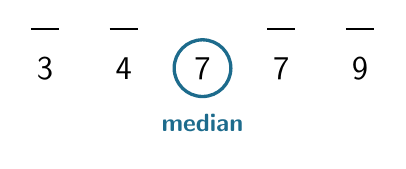
\begin{tikzpicture}[baseline=-1mm]\node[font=\large] (n0) at (0,0) {3};\node[font=\large] (n1) at (1,0) {4};\node[font=\large] (n2) at (2,0) {7};\node[font=\large] (n3) at (3,0) {7};\node[font=\large] (n4) at (4,0) {9};\draw[thick] (-0.18,0.5) -- (0.18,0.5);\draw[thick] (0.82,0.5) -- (1.18,0.5);\draw[thick] (2.82,0.5) -- (3.18,0.5);\draw[thick] (3.82,0.5) -- (4.18,0.5);\draw[accent, very thick] (2,0) circle (0.36);\node[accent, font=\small\bfseries] at (2,-0.7) {median};\end{tikzpicture}\hspace{8mm} Median $= 7$

\textbf{Mean:} $3 + 4 + 7 + 7 + 9 = 30$, \quad and there are 5 numbers, \quad so $30 \div 5 = 6$. \quad Mean $= 6$

\subsection*{When there is an even number of values}
The dashes meet \textbf{between two numbers}. The median is \textbf{halfway} between them.\par
\hspace*{10mm}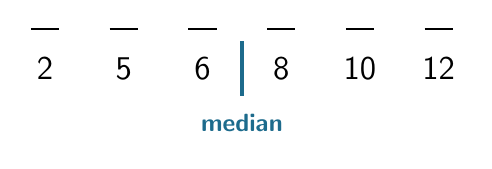
\begin{tikzpicture}[baseline=-1mm]\node[font=\large] (n0) at (0,0) {2};\node[font=\large] (n1) at (1,0) {5};\node[font=\large] (n2) at (2,0) {6};\node[font=\large] (n3) at (3,0) {8};\node[font=\large] (n4) at (4,0) {10};\node[font=\large] (n5) at (5,0) {12};\draw[thick] (-0.18,0.5) -- (0.18,0.5);\draw[thick] (0.82,0.5) -- (1.18,0.5);\draw[thick] (1.82,0.5) -- (2.18,0.5);\draw[thick] (2.82,0.5) -- (3.18,0.5);\draw[thick] (3.82,0.5) -- (4.18,0.5);\draw[thick] (4.82,0.5) -- (5.18,0.5);\draw[accent, very thick] (2.5,-0.35) -- (2.5,0.35);\node[accent, font=\small\bfseries] at (2.5,-0.7) {median};\end{tikzpicture}\hspace{8mm} Median $= \dfrac{6 + 8}{2} = 7$

\begin{rememberbox}
\textbf{Always order the numbers first} for the median. The mean and median can be decimals, e.g. 7.5.
\end{rememberbox}

\newpage\normalsize
\banner{5}{Mean, Median and Mode}{Practice}{accent}
{\large\textbf{Order the numbers first, then find the answer.}} {\color{muted}Show your working in each box.}\par\vspace{1mm}
\begin{tcbraster}[raster columns=2, raster column skip=4mm, raster row skip=3mm]
\pbox{1}{3.3cm}{\raggedright{\large Find the \textbf{mode}:}\par\vspace{1mm}{\large 3, 5, 5, 6, 8}\par\vfill Mode $=$\ \ansline{0.55}}
\pbox{2}{3.3cm}{\raggedright{\large Find the \textbf{mode}:}\par\vspace{1mm}{\large 4, 9, 7, 2, 7, 4, 7}\par\vfill Mode $=$\ \ansline{0.55}}
\pbox{3}{3.3cm}{\raggedright{\large Find the \textbf{median}:}\par\vspace{1mm}{\large 2, 4, 7, 9, 10}\par\vfill Median $=$\ \ansline{0.55}}
\pbox{4}{3.3cm}{\raggedright{\large Find the \textbf{median}:}\par\vspace{1mm}{\large 11, 3, 8, 5, 6}\par\vfill Median $=$\ \ansline{0.55}}
\pbox{5}{3.3cm}{\raggedright{\large Find the \textbf{median}:}\par\vspace{1mm}{\large 21, 18, 25, 18, 30, 22, 19}\par\vfill Median $=$\ \ansline{0.55}}
\pbox{6}{3.3cm}{\raggedright{\large Find the \textbf{median}:}\par\vspace{1mm}{\large 4, 6, 9, 12}\par\vfill Median $=$\ \ansline{0.55}}
\pbox{7}{3.3cm}{\raggedright{\large Find the \textbf{median}:}\par\vspace{1mm}{\large 15, 10, 20, 25, 30, 5}\par\vfill Median $=$\ \ansline{0.55}}
\pbox{8}{3.3cm}{\raggedright{\large Find the \textbf{mean}:}\par\vspace{1mm}{\large 2, 4, 6, 8}\par\vfill Mean $=$\ \ansline{0.55}}
\pbox{9}{3.3cm}{\raggedright{\large Find the \textbf{mean}:}\par\vspace{1mm}{\large 5, 7, 9, 3, 6}\par\vfill Mean $=$\ \ansline{0.55}}
\pbox{10}{3.3cm}{\raggedright{\large Find the \textbf{mean}:}\par\vspace{1mm}{\large 10, 12, 14, 16, 18}\par\vfill Mean $=$\ \ansline{0.55}}
\pbox{11}{3.3cm}{\raggedright{\large Find the \textbf{mean}:}\par\vspace{1mm}{\large 3, 8, 6, 7}\par\vfill Mean $=$\ \ansline{0.55}}
\pbox{12}{3.3cm}{\raggedright{\large Find the \textbf{mean}:}\par\vspace{1mm}{\large 12, 15, 9, 20, 14, 8}\par\vfill Mean $=$\ \ansline{0.55}}
\end{tcbraster}
\vfill\centerline{\color{good}\bfseries \ding{51}\ Check your answers at the back. Fix any you got wrong.}
\newpage
\banner{6}{Range and Quartiles}{Learn}{accent}
\begin{tcolorbox}[enhanced, colback=accentlight, colframe=accent, boxrule=0pt, leftrule=1.5mm, arc=0mm, top=1.5mm, bottom=1.5mm]\textbf{Goal:} I can find the range, LQ, UQ and IQR of a set of data\end{tcolorbox}
\large

The \textbf{spread} tells you how spread out the data is.

\begin{center}
\renewcommand{\arraystretch}{1.4}
\begin{tabular}{|p{4.2cm}|p{11.2cm}|}
\hline
\textbf{Range} & Biggest value $-$ smallest value. \\ \hline
\textbf{Lower quartile (LQ)} & The middle of the \textbf{lower half} of the data. \\ \hline
\textbf{Upper quartile (UQ)} & The middle of the \textbf{upper half} of the data. \\ \hline
\textbf{Interquartile range (IQR)} & $\text{UQ} - \text{LQ}$. The spread of the middle half of the data. \\ \hline
\end{tabular}
\end{center}

\subsection*{Example: 9, 2, 14, 5, 11, 3, 18, 8, 15, 6, 12}
\textbf{Step 1: put the numbers in order.} \quad 2, 3, 5, 6, 8, 9, 11, 12, 14, 15, 18

\textbf{Range:} $18 - 2 = 16$

\textbf{Step 2: find the median.} Draw dashes over the numbers from each end until you reach the middle.\par
\hspace*{6mm}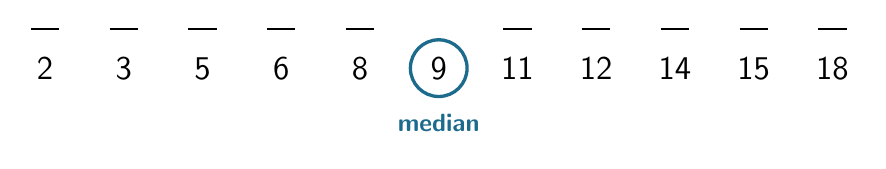
\begin{tikzpicture}[baseline=-1mm]\node[font=\large] (n0) at (0,0) {2};\node[font=\large] (n1) at (1,0) {3};\node[font=\large] (n2) at (2,0) {5};\node[font=\large] (n3) at (3,0) {6};\node[font=\large] (n4) at (4,0) {8};\node[font=\large] (n5) at (5,0) {9};\node[font=\large] (n6) at (6,0) {11};\node[font=\large] (n7) at (7,0) {12};\node[font=\large] (n8) at (8,0) {14};\node[font=\large] (n9) at (9,0) {15};\node[font=\large] (n10) at (10,0) {18};\draw[thick] (-0.18,0.5) -- (0.18,0.5);\draw[thick] (0.82,0.5) -- (1.18,0.5);\draw[thick] (1.82,0.5) -- (2.18,0.5);\draw[thick] (2.82,0.5) -- (3.18,0.5);\draw[thick] (3.82,0.5) -- (4.18,0.5);\draw[thick] (5.82,0.5) -- (6.18,0.5);\draw[thick] (6.82,0.5) -- (7.18,0.5);\draw[thick] (7.82,0.5) -- (8.18,0.5);\draw[thick] (8.82,0.5) -- (9.18,0.5);\draw[thick] (9.82,0.5) -- (10.18,0.5);\draw[accent, very thick] (5,0) circle (0.36);\node[accent, font=\small\bfseries] at (5,-0.7) {median};\end{tikzpicture}

\textbf{Step 3: find the quartiles.} The median splits the data into two halves (the median is \textbf{not} in either half).
In each half, cross out the dashes from each end until you reach the middle of that half.\par
\hspace*{6mm}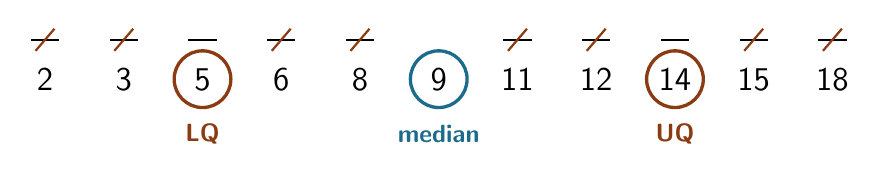
\begin{tikzpicture}[baseline=-1mm]\node[font=\large] (n0) at (0,0) {2};\node[font=\large] (n1) at (1,0) {3};\node[font=\large] (n2) at (2,0) {5};\node[font=\large] (n3) at (3,0) {6};\node[font=\large] (n4) at (4,0) {8};\node[font=\large] (n5) at (5,0) {9};\node[font=\large] (n6) at (6,0) {11};\node[font=\large] (n7) at (7,0) {12};\node[font=\large] (n8) at (8,0) {14};\node[font=\large] (n9) at (9,0) {15};\node[font=\large] (n10) at (10,0) {18};\draw[thick] (-0.18,0.5) -- (0.18,0.5);\draw[checkcol, thick] (-0.12,0.36) -- (0.12,0.64);\draw[thick] (0.82,0.5) -- (1.18,0.5);\draw[checkcol, thick] (0.88,0.36) -- (1.12,0.64);\draw[thick] (1.82,0.5) -- (2.18,0.5);\draw[thick] (2.82,0.5) -- (3.18,0.5);\draw[checkcol, thick] (2.88,0.36) -- (3.12,0.64);\draw[thick] (3.82,0.5) -- (4.18,0.5);\draw[checkcol, thick] (3.88,0.36) -- (4.12,0.64);\draw[thick] (5.82,0.5) -- (6.18,0.5);\draw[checkcol, thick] (5.88,0.36) -- (6.12,0.64);\draw[thick] (6.82,0.5) -- (7.18,0.5);\draw[checkcol, thick] (6.88,0.36) -- (7.12,0.64);\draw[thick] (7.82,0.5) -- (8.18,0.5);\draw[thick] (8.82,0.5) -- (9.18,0.5);\draw[checkcol, thick] (8.88,0.36) -- (9.12,0.64);\draw[thick] (9.82,0.5) -- (10.18,0.5);\draw[checkcol, thick] (9.88,0.36) -- (10.12,0.64);\draw[accent, very thick] (5,0) circle (0.36);\node[accent, font=\small\bfseries] at (5,-0.7) {median};\draw[checkcol, very thick] (2,0) circle (0.36);\node[checkcol, font=\small\bfseries] at (2,-0.7) {LQ};\draw[checkcol, very thick] (8,0) circle (0.36);\node[checkcol, font=\small\bfseries] at (8,-0.7) {UQ};\end{tikzpicture}

\textbf{LQ} $= 5$, \quad \textbf{UQ} $= 14$, \quad \textbf{IQR} $= 14 - 5 = 9$

\begin{rememberbox}
If a half has an \textbf{even} number of values, the quartile is \textbf{halfway} between the two middle numbers ---
the same as for the median.
\end{rememberbox}

\newpage\normalsize
\banner{6}{Range and Quartiles}{Practice}{accent}
{\large\textbf{Order the numbers first. Use the dash method for the median and quartiles.}} {\color{muted}Show your working in each box.}\par\vspace{1mm}
\begin{tcbraster}[raster columns=6, raster column skip=4mm, raster row skip=3mm]
\pbox[raster multicolumn=2]{1}{3.0cm}{\raggedright{\large Find the \textbf{range}:}\par\vspace{1mm}{\large 4, 9, 2, 12, 7}\par\vfill Range $=$\ \ansline{0.55}}
\pbox[raster multicolumn=2]{2}{3.0cm}{\raggedright{\large Find the \textbf{range}:}\par\vspace{1mm}{\large 15, 22, 18, 30, 11}\par\vfill Range $=$\ \ansline{0.55}}
\pbox[raster multicolumn=2]{3}{3.0cm}{\raggedright{\large Find the \textbf{range}:}\par\vspace{1mm}{\large 35, 42, 28, 50, 47, 31}\par\vfill Range $=$\ \ansline{0.55}}
\pbox[raster multicolumn=3]{4}{5.6cm}{\raggedright{\large 2, 4, 5, 7, 9, 10, 12}\par\vspace{2mm}Median $=$\ \ansline{0.45}\par\vfill LQ $=$\ \ansline{0.45}\par\vfill UQ $=$\ \ansline{0.45}\par\vfill IQR $=$\ \ansline{0.45}}
\pbox[raster multicolumn=3]{5}{5.6cm}{\raggedright{\large 12, 5, 9, 20, 15, 7, 18}\par\vspace{2mm}Median $=$\ \ansline{0.45}\par\vfill LQ $=$\ \ansline{0.45}\par\vfill UQ $=$\ \ansline{0.45}\par\vfill IQR $=$\ \ansline{0.45}}
\pbox[raster multicolumn=3]{6}{5.6cm}{\raggedright{\large 3, 6, 8, 9, 11, 14, 15, 18, 20, 22, 25}\par\vspace{2mm}Median $=$\ \ansline{0.45}\par\vfill LQ $=$\ \ansline{0.45}\par\vfill UQ $=$\ \ansline{0.45}\par\vfill IQR $=$\ \ansline{0.45}}
\pbox[raster multicolumn=3]{7}{5.6cm}{\raggedright{\large 45, 32, 50, 38, 41, 29, 36, 47, 40, 33, 52}\par\vspace{2mm}Median $=$\ \ansline{0.45}\par\vfill LQ $=$\ \ansline{0.45}\par\vfill UQ $=$\ \ansline{0.45}\par\vfill IQR $=$\ \ansline{0.45}}
\pbox[raster multicolumn=3]{8}{5.6cm}{\raggedright{\large 10, 12, 15, 16, 18, 21, 22, 25, 30}\par\vspace{2mm}Median $=$\ \ansline{0.45}\par\vfill LQ $=$\ \ansline{0.45}\par\vfill UQ $=$\ \ansline{0.45}\par\vfill IQR $=$\ \ansline{0.45}}
\pbox[raster multicolumn=3]{9}{5.6cm}{\raggedright{\large 1, 3, 4, 6, 7, 9, 10, 12}\par\vspace{2mm}Median $=$\ \ansline{0.45}\par\vfill LQ $=$\ \ansline{0.45}\par\vfill UQ $=$\ \ansline{0.45}\par\vfill IQR $=$\ \ansline{0.45}}
\end{tcbraster}
\vfill\centerline{\color{good}\bfseries \ding{51}\ Check your answers at the back. Fix any you got wrong.}
\newpage
\banner{\ding{51}}{Skill Checks}{Teacher marks}{checkcol}
{\large Name: \fillline{8cm}}\hfill\par\vspace{1mm}
Do these \textbf{on your own --- no notes}. Show your working, and write your final answer on the line.
\checkhead{1}{Data Sources and Types}{Circle the correct answer.}{4}
\begin{tcbraster}[raster columns=4, raster column skip=3mm]
\kbox{1}{4.9cm}{{\normalsize Rawiri reads house prices in a newspaper.}\par\vfill {\small Circle one:}\par\vspace{1mm}{\footnotesize\raggedright \fbox{\strut\ Primary\ }\par\vspace{1mm}\fbox{\strut\ Secondary\ }}}
\kbox{2}{4.9cm}{{\normalsize Type of data: \textbf{number of siblings}}\par\vfill {\small Circle one:}\par\vspace{1mm}{\footnotesize\raggedright \fbox{\strut\ Categorical\ }\par\vspace{1mm}\fbox{\strut\ Discrete numerical\ }\par\vspace{1mm}\fbox{\strut\ Continuous numerical\ }}}
\kbox{3}{4.9cm}{{\normalsize Type of data: \textbf{favourite colour}}\par\vfill {\small Circle one:}\par\vspace{1mm}{\footnotesize\raggedright \fbox{\strut\ Categorical\ }\par\vspace{1mm}\fbox{\strut\ Discrete numerical\ }\par\vspace{1mm}\fbox{\strut\ Continuous numerical\ }}}
\kbox{4}{4.9cm}{{\normalsize Type of data: \textbf{homework time}}\par\vfill {\small Circle one:}\par\vspace{1mm}{\footnotesize\raggedright \fbox{\strut\ Categorical\ }\par\vspace{1mm}\fbox{\strut\ Discrete numerical\ }\par\vspace{1mm}\fbox{\strut\ Continuous numerical\ }}}
\end{tcbraster}
\checkhead{2}{Data Displays}{Use: pie chart, bar graph, histogram, pictograph, line graph.}{4}
\begin{tcbraster}[raster columns=4, raster column skip=3mm]
\kbox{1}{4.6cm}{\par\centering 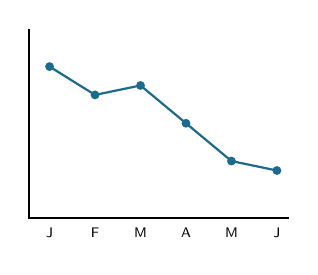
\begin{tikzpicture}[x=0.3300cm,y=0.2400cm]\draw[thick] (0,10) -- (0,0) -- (10,0);\draw[accent, thick] (0.8,8) -- (2.55,6.5) -- (4.3,7) -- (6.05,5) -- (7.8,3) -- (9.55,2.5);\fill[accent] (0.8,8) circle (1.6pt);\fill[accent] (2.55,6.5) circle (1.6pt);\fill[accent] (4.3,7) circle (1.6pt);\fill[accent] (6.05,5) circle (1.6pt);\fill[accent] (7.8,3) circle (1.6pt);\fill[accent] (9.55,2.5) circle (1.6pt);\node[below, font=\tiny] at (0.8,0) {J};\node[below, font=\tiny] at (2.55,0) {F};\node[below, font=\tiny] at (4.3,0) {M};\node[below, font=\tiny] at (6.05,0) {A};\node[below, font=\tiny] at (7.8,0) {M};\node[below, font=\tiny] at (9.55,0) {J};\end{tikzpicture}\par\vfill\raggedright This is a\ \ansline{0.6}}
\kbox{2}{4.6cm}{\par\centering 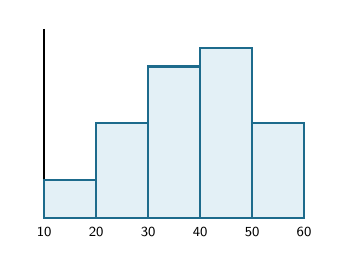
\begin{tikzpicture}[x=0.3300cm,y=0.2400cm]\draw[thick] (0,10) -- (0,0) -- (10,0);\filldraw[fill=accentlight, draw=accent, thick] (0,0) rectangle (2,2);\filldraw[fill=accentlight, draw=accent, thick] (2,0) rectangle (4,5);\filldraw[fill=accentlight, draw=accent, thick] (4,0) rectangle (6,8);\filldraw[fill=accentlight, draw=accent, thick] (6,0) rectangle (8,9);\filldraw[fill=accentlight, draw=accent, thick] (8,0) rectangle (10,5);\node[below, font=\tiny] at (0,0) {10};\node[below, font=\tiny] at (2,0) {20};\node[below, font=\tiny] at (4,0) {30};\node[below, font=\tiny] at (6,0) {40};\node[below, font=\tiny] at (8,0) {50};\node[below, font=\tiny] at (10,0) {60};\end{tikzpicture}\par\vfill\raggedright This is a\ \ansline{0.6}}
\kbox{3}{4.6cm}{{\normalsize Best display to show how a baby's weight changed each month for a year?}\par\vfill \ansline{0.95}}
\kbox{4}{4.6cm}{{\normalsize Best display to show the share of a budget spent on rent, food and power?}\par\vfill \ansline{0.95}}
\end{tcbraster}
\checkhead{3}{Scatter Plots}{Use the scatter plot.}{3}
\begin{tcbraster}[raster columns=4, raster column skip=3mm]
\kbox[raster multicolumn=4]{1}{7.5cm}{\textbf{Age and height of 12 children}\par\vspace{1mm}\begin{minipage}[t]{0.52\linewidth}\vspace{0pt}\hspace*{9mm}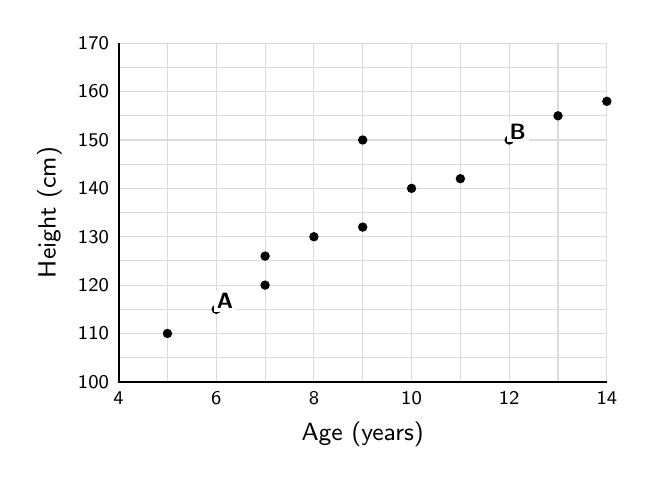
\begin{tikzpicture}[x=0.62000cm,y=0.06143cm, baseline=(current bounding box.north)]\draw[black!14] (0,0) -- (0,70);\node[below, font=\scriptsize] at (0,0) {4};\draw[black!14] (1,0) -- (1,70);\draw[black!14] (2,0) -- (2,70);\node[below, font=\scriptsize] at (2,0) {6};\draw[black!14] (3,0) -- (3,70);\draw[black!14] (4,0) -- (4,70);\node[below, font=\scriptsize] at (4,0) {8};\draw[black!14] (5,0) -- (5,70);\draw[black!14] (6,0) -- (6,70);\node[below, font=\scriptsize] at (6,0) {10};\draw[black!14] (7,0) -- (7,70);\draw[black!14] (8,0) -- (8,70);\node[below, font=\scriptsize] at (8,0) {12};\draw[black!14] (9,0) -- (9,70);\draw[black!14] (10,0) -- (10,70);\node[below, font=\scriptsize] at (10,0) {14};\draw[black!14] (0,0) -- (10,0);\node[left, font=\scriptsize] at (0,0) {100};\draw[black!14] (0,5) -- (10,5);\draw[black!14] (0,10) -- (10,10);\node[left, font=\scriptsize] at (0,10) {110};\draw[black!14] (0,15) -- (10,15);\draw[black!14] (0,20) -- (10,20);\node[left, font=\scriptsize] at (0,20) {120};\draw[black!14] (0,25) -- (10,25);\draw[black!14] (0,30) -- (10,30);\node[left, font=\scriptsize] at (0,30) {130};\draw[black!14] (0,35) -- (10,35);\draw[black!14] (0,40) -- (10,40);\node[left, font=\scriptsize] at (0,40) {140};\draw[black!14] (0,45) -- (10,45);\draw[black!14] (0,50) -- (10,50);\node[left, font=\scriptsize] at (0,50) {150};\draw[black!14] (0,55) -- (10,55);\draw[black!14] (0,60) -- (10,60);\node[left, font=\scriptsize] at (0,60) {160};\draw[black!14] (0,65) -- (10,65);\draw[black!14] (0,70) -- (10,70);\node[left, font=\scriptsize] at (0,70) {170};\draw[thick] (0,70) -- (0,0) -- (10,0);\node[below=11pt, font=\small] at (5,0) {Age (years)};\node[rotate=90, above=17pt, font=\small] at (0,35) {Height (cm)};\fill (1,10) circle (1.7pt);\fill (2,15) circle (1.7pt);\fill (3,20) circle (1.7pt);\fill (3,26) circle (1.7pt);\fill (4,30) circle (1.7pt);\fill (5,32) circle (1.7pt);\fill (6,40) circle (1.7pt);\fill (7,42) circle (1.7pt);\fill (8,50) circle (1.7pt);\fill (9,55) circle (1.7pt);\fill (5,50) circle (1.7pt);\fill (10,58) circle (1.7pt);\node[above right=-1pt, font=\footnotesize\bfseries, fill=white, inner sep=1pt] at (2,15) {A};\node[above right=-1pt, font=\footnotesize\bfseries, fill=white, inner sep=1pt] at (8,50) {B};\end{tikzpicture}\end{minipage}\hfill\begin{minipage}[t]{0.46\linewidth}\vspace{0pt}{\small\textbf{(a)} Describe point \textbf{A} in context.}\par\vspace{4mm}\ansline{1}\par\vspace{1.5mm}{\small\textbf{(b)} Describe point \textbf{B} in context.}\par\vspace{4mm}\ansline{1}\par\vspace{1.5mm}{\small\textbf{(c)} Describe the strength and direction of the relationship.}\par\vspace{4mm}\ansline{1}\end{minipage}}
\end{tcbraster}
\newpage
\banner{\ding{51}}{Skill Checks}{Continued}{checkcol}
{\large Name: \fillline{8cm}}\hfill\fcolorbox{checkcol}{white}{\parbox[c][8mm][c]{4.2cm}{\centering\color{checkcol}\bfseries\large Total: \underline{\hspace{9mm}} / 22}}\par\vspace{1mm}
Do these \textbf{on your own --- no notes}. Show your working, and write your final answer on the line.
\checkhead{4}{Lines of Best Fit}{Use a ruler.}{3}
\begin{tcbraster}[raster columns=4, raster column skip=3mm]
\kbox[raster multicolumn=4]{1}{6.9cm}{\textbf{Distance from school and travel time for 12 students}\par\vspace{1mm}\begin{minipage}[t]{0.52\linewidth}\vspace{0pt}\hspace*{9mm}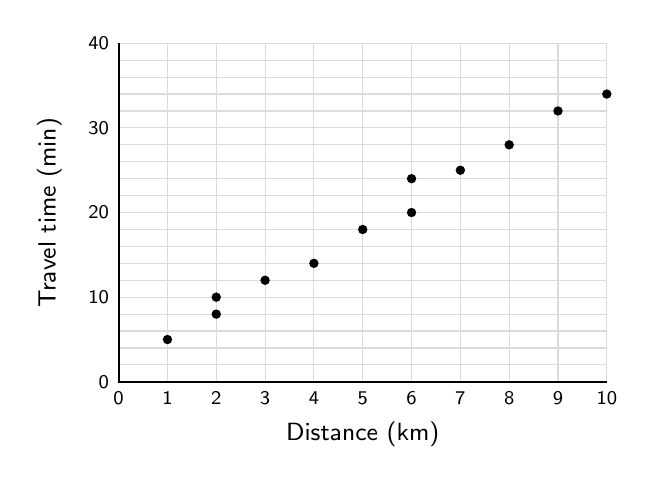
\begin{tikzpicture}[x=0.62000cm,y=0.10750cm, baseline=(current bounding box.north)]\draw[black!14] (0,0) -- (0,40);\node[below, font=\scriptsize] at (0,0) {0};\draw[black!14] (1,0) -- (1,40);\node[below, font=\scriptsize] at (1,0) {1};\draw[black!14] (2,0) -- (2,40);\node[below, font=\scriptsize] at (2,0) {2};\draw[black!14] (3,0) -- (3,40);\node[below, font=\scriptsize] at (3,0) {3};\draw[black!14] (4,0) -- (4,40);\node[below, font=\scriptsize] at (4,0) {4};\draw[black!14] (5,0) -- (5,40);\node[below, font=\scriptsize] at (5,0) {5};\draw[black!14] (6,0) -- (6,40);\node[below, font=\scriptsize] at (6,0) {6};\draw[black!14] (7,0) -- (7,40);\node[below, font=\scriptsize] at (7,0) {7};\draw[black!14] (8,0) -- (8,40);\node[below, font=\scriptsize] at (8,0) {8};\draw[black!14] (9,0) -- (9,40);\node[below, font=\scriptsize] at (9,0) {9};\draw[black!14] (10,0) -- (10,40);\node[below, font=\scriptsize] at (10,0) {10};\draw[black!14] (0,0) -- (10,0);\node[left, font=\scriptsize] at (0,0) {0};\draw[black!14] (0,2) -- (10,2);\draw[black!14] (0,4) -- (10,4);\draw[black!14] (0,6) -- (10,6);\draw[black!14] (0,8) -- (10,8);\draw[black!14] (0,10) -- (10,10);\node[left, font=\scriptsize] at (0,10) {10};\draw[black!14] (0,12) -- (10,12);\draw[black!14] (0,14) -- (10,14);\draw[black!14] (0,16) -- (10,16);\draw[black!14] (0,18) -- (10,18);\draw[black!14] (0,20) -- (10,20);\node[left, font=\scriptsize] at (0,20) {20};\draw[black!14] (0,22) -- (10,22);\draw[black!14] (0,24) -- (10,24);\draw[black!14] (0,26) -- (10,26);\draw[black!14] (0,28) -- (10,28);\draw[black!14] (0,30) -- (10,30);\node[left, font=\scriptsize] at (0,30) {30};\draw[black!14] (0,32) -- (10,32);\draw[black!14] (0,34) -- (10,34);\draw[black!14] (0,36) -- (10,36);\draw[black!14] (0,38) -- (10,38);\draw[black!14] (0,40) -- (10,40);\node[left, font=\scriptsize] at (0,40) {40};\draw[thick] (0,40) -- (0,0) -- (10,0);\node[below=11pt, font=\small] at (5,0) {Distance (km)};\node[rotate=90, above=17pt, font=\small] at (0,20) {Travel time (min)};\fill (1,5) circle (1.7pt);\fill (2,8) circle (1.7pt);\fill (2,10) circle (1.7pt);\fill (3,12) circle (1.7pt);\fill (4,14) circle (1.7pt);\fill (5,18) circle (1.7pt);\fill (6,20) circle (1.7pt);\fill (6,24) circle (1.7pt);\fill (7,25) circle (1.7pt);\fill (8,28) circle (1.7pt);\fill (9,32) circle (1.7pt);\fill (10,34) circle (1.7pt);\end{tikzpicture}\end{minipage}\hfill\begin{minipage}[t]{0.46\linewidth}\vspace{0pt}{\small\textbf{(a)} Draw a line of best fit on the graph.}\par\vspace{1.5mm}{\small\textbf{(b)} Predict the travel time for a student who lives 5\,km from school.}\par\vspace{4mm}\ansline{1}\par\vspace{1.5mm}{\small\textbf{(c)} Predict how far away a student lives if their trip takes 30 minutes.}\par\vspace{4mm}\ansline{1}\end{minipage}}
\end{tcbraster}
\checkhead{5}{Mean, Median and Mode}{Show your working.}{4}
\begin{tcbraster}[raster columns=4, raster column skip=3mm]
\kbox{1}{3.7cm}{\raggedright{\normalsize Find the \textbf{mode}:}\par\vspace{1mm}{\normalsize 6, 3, 8, 3, 9, 3}\par\vfill Mode $=$\ \ansline{0.55}}
\kbox{2}{3.7cm}{\raggedright{\normalsize Find the \textbf{median}:}\par\vspace{1mm}{\normalsize 9, 4, 12, 7, 15}\par\vfill Median $=$\ \ansline{0.55}}
\kbox{3}{3.7cm}{\raggedright{\normalsize Find the \textbf{median}:}\par\vspace{1mm}{\normalsize 3, 8, 10, 13}\par\vfill Median $=$\ \ansline{0.55}}
\kbox{4}{3.7cm}{\raggedright{\normalsize Find the \textbf{mean}:}\par\vspace{1mm}{\normalsize 4, 9, 5, 10, 7}\par\vfill Mean $=$\ \ansline{0.55}}
\end{tcbraster}
\checkhead{6}{Range and Quartiles}{Order the numbers first.}{4}
\begin{tcbraster}[raster columns=4, raster column skip=3mm]
\kbox{1}{4.6cm}{\raggedright{\normalsize Find the \textbf{range}:}\par\vspace{1mm}{\normalsize 8, 3, 14, 6, 11}\par\vfill Range $=$\ \ansline{0.55}}
\kbox[raster multicolumn=3]{2}{4.6cm}{\raggedright{\normalsize 13, 4, 9, 6, 15, 7, 12}\par\vspace{2mm}LQ $=$\ \ansline{0.45}\par\vfill UQ $=$\ \ansline{0.45}\par\vfill IQR $=$\ \ansline{0.45}}
\end{tcbraster}
\newpage
\setlength{\multicolsep}{3pt plus 1pt}\titlespacing*{\subsection}{0pt}{6pt}{2pt}
{\LARGE\bfseries\color{accent} Answers to the Practice Questions}\par\vspace{1mm}
{\small\color{muted} Terms can be in a different order and still be right --- e.g. $2b + 3a$ is the same as $3a + 2b$.}\par
\subsection*{1. Data Sources and Types}
\begin{multicols}{2}\begin{enumerate}[nosep, label=\arabic*., start=1]
\item Primary
\item Secondary
\item Primary
\item Secondary
\item Secondary
\item Categorical
\item Discrete numerical
\item Continuous numerical
\item Categorical
\item Discrete numerical
\item Continuous numerical
\item Discrete numerical
\end{enumerate}\end{multicols}

\subsection*{2. Data Displays}
\begin{multicols}{3}\begin{enumerate}[nosep, label=\arabic*., start=1]
\item Bar graph
\item Pie chart
\item Line graph
\item Histogram
\item Pictograph
\item Histogram
\end{enumerate}\end{multicols}
\begin{multicols}{2}\begin{enumerate}[nosep, label=\arabic*., start=7]
\item Line graph
\item Pie chart
\item Bar graph
\item Histogram
\item Pictograph
\item Line graph
\end{enumerate}\end{multicols}

\subsection*{3. Scatter Plots}
\begin{enumerate}[nosep, label=\arabic*., start=1]
\item \textbf{(a)} Point A is a student who studied for 2 hours and scored 40 marks.\quad \textbf{(b)} Point B is a student who studied for 5 hours and scored 65 marks.\quad \textbf{(c)} Point E is a student who studied for 9 hours and scored 40 marks.\quad \textbf{(d)} D\quad \textbf{(e)} Moderate positive.
\end{enumerate}
\begin{multicols}{3}\begin{enumerate}[nosep, label=\arabic*., start=2]
\item strong positive
\item moderate negative
\item no relationship
\item weak positive
\item strong negative
\item moderate positive
\end{enumerate}\end{multicols}

\subsection*{4. Lines of Best Fit}
\begin{enumerate}[nosep, label=\arabic*., start=1]
\item \textbf{(a)} A straight line through the middle of the points, with about the same number of points above and below it.\quad \textbf{(b)} About \$24\,000 (accept \$22\,000 to \$26\,000).\quad \textbf{(c)} About \$12\,000 (accept \$10\,000 to \$14\,000).\quad \textbf{(d)} About 5.5 years (accept 4.5 to 6.5 years).
\item \textbf{(a)} A straight line through the middle of the points, with about the same number of points above and below it.\quad \textbf{(b)} About 36 (accept 28 to 44).\quad \textbf{(c)} About 85 (accept 77 to 93).\quad \textbf{(d)} About 21$^\circ$C (accept 19 to 23$^\circ$C).
\end{enumerate}

\subsection*{5. Mean, Median and Mode}
\begin{multicols}{4}\begin{enumerate}[nosep, label=\arabic*., start=1]
\item 5
\item 7
\item 7
\item 6
\item 21
\item 7.5
\item 17.5
\item 5
\item 6
\item 14
\item 6
\item 13
\end{enumerate}\end{multicols}

\subsection*{6. Range and Quartiles}
\begin{multicols}{4}\begin{enumerate}[nosep, label=\arabic*., start=1]
\item 10
\item 19
\item 22
\end{enumerate}\end{multicols}
\begin{enumerate}[nosep, label=\arabic*., start=4]
\item Median = 7, LQ = 4, UQ = 10, IQR = 6
\item Median = 12, LQ = 7, UQ = 18, IQR = 11
\item Median = 14, LQ = 8, UQ = 20, IQR = 12
\item Median = 40, LQ = 33, UQ = 47, IQR = 14
\item Median = 18, LQ = 13.5, UQ = 23.5, IQR = 10
\item Median = 6.5, LQ = 3.5, UQ = 9.5, IQR = 6
\end{enumerate}

\end{document}
